% CVPR 2022 Paper Template
% based on the CVPR template provided by Ming-Ming Cheng (https://github.com/MCG-NKU/CVPR_Template)
% modified and extended by Stefan Roth (stefan.roth@NOSPAMtu-darmstadt.de)

\documentclass[10pt,twocolumn,letterpaper]{article}

%%%%%%%%% PAPER TYPE  - PLEASE UPDATE FOR FINAL VERSION %%%%%%%%%
%\usepackage[review]{cvpr}      % To produce the REVIEW version
%\usepackage{cvpr}              % To produce the CAMERA-READY version
\usepackage[pagenumbers]{cvpr} % To force page numbers, e.g. for an arXiv version

% Include other packages here, before hyperref.
\usepackage{graphicx}
\usepackage{amsmath}
\usepackage{amssymb}
\usepackage{booktabs}
\usepackage{float}
\usepackage{arydshln}
\usepackage{enumitem}


% It is strongly recommended to use hyperref, especially for the review version.
% hyperref with option pagebackref eases the reviewers' job.
% Please disable hyperref *only* if you encounter grave issues, e.g. with the
% file validation for the camera-ready version.
%
% If you comment hyperref and then uncomment it, you should delete
% ReviewTempalte.aux before re-running LaTeX.
% (Or just hit 'q' on the first LaTeX run, let it finish, and you
%  should be clear).
\usepackage[pagebackref,breaklinks,colorlinks]{hyperref}


% Support for easy cross-referencing
\usepackage[capitalize]{cleveref}
\crefname{section}{Sec.}{Secs.}
\Crefname{section}{Section}{Sections}
\Crefname{table}{Table}{Tables}
\crefname{table}{Tab.}{Tabs.}

\raggedbottom
\begin{document}

%%%%%%%%% TITLE - PLEASE UPDATE %%%%%%%%%
\title{DLP Lab7: Policy-Based Reinforcement Learning}

\author{Yi-Hsiang Ho, 111550106
}
\maketitle

%%%%%%%%% BODY TEXT %%%%%%%%%

\section{Introduction}
\label{sec:intro}

Continuous control in high-dimensional action spaces presents significant
challenges regarding sample efficiency, exploration, and training stability.
In this report, I evaluate on-policy methods, specifically \textbf{Advantage
  Actor-Critic (A2C)} and \textbf{Proximal Policy Optimization (PPO)}, on the
continuous tasks \textbf{Pendulum-v1} and \textbf{Walker2d-v5}.

To achieve stable policy convergence, my implementation highlights the
critical role of specific stabilization techniques:
\begin{itemize}[itemsep=-3pt]
  \item \textbf{Gradient Clipping} (\verb|clip_grad_norm_|): Essential
        for preventing extreme parameter shifts in both A2C and PPO, especially in
        bounding policy and value updates against gradient explosion.
  \item \textbf{Observation Normalization}: The single most critical continuous
        control trick for high-dimensional states (e.g., Walker2d-v5), normalizing
        state bounds dynamically to avoid gradient saturation.
  \item \textbf{Clipped Surrogate Objective \& GAE}: Implemented in PPO to
        constrain policy update scales and balance return estimation bias and
        variance.
\end{itemize}

Additionally, I conducted ablation studies incorporating both a learning rate
scheduler and advantage normalization in Task 3. The empirical results
demonstrate that integrating these techniques alongside observation normalization 
yields significant synergistic improvements, achieving the highest returns 
and superior training stability compared to using observation normalization alone.

\section{Implementation}
\label{sec:implementation}

\subsection{Stochastic Policy Gradient and TD Error in A2C}
\label{subsec:impl_a2c}

\paragraph{Mathematical Concepts:}
Advantage Actor-Critic (A2C) is an on-policy method that optimizes a
parameterized policy (the Actor) $\pi_\theta(a|s)$ using the stochastic
policy gradient, while using a state-value function estimator (the Critic)
$V_\phi(s)$ as a baseline to reduce gradient variance. The objective
function $J(\theta)$ representing the expected return is maximized by
updating policy parameters $\theta$ in the direction of the policy
gradient:
\begin{equation}
  \nabla_\theta J(\theta) = \mathbb{E}_{s_t, a_t \sim \pi_\theta} \left[ \nabla_\theta \log \pi_\theta(a_t | s_t) A(s_t, a_t) \right]
  \label{eq:pg}
\end{equation}
where $A(s_t, a_t)$ is the advantage function. In A2C, the advantage is
estimated using the 1-step Temporal Difference (TD) error $\delta_t$:
\begin{equation}
  A(s_t, a_t) \approx \delta_t = Q(s_t, a_t) - V_\phi(s_t)
  \label{eq:advantage}
\end{equation}
where the target action-value $Q(s_t, a_t)$ is computed from the 1-step
empirical bootstrap:
\begin{equation}
  Q(s_t, a_t) = r_t + \gamma V_\phi(s_{t+1}) (1 - d_t)
  \label{eq:q_val}
\end{equation}
where $\gamma$ is the discount factor and $d_t$ is the environment
termination/truncation boolean flag (\texttt{done}). The Critic
parameters $\phi$ are optimized by minimizing MSE between the
state-value prediction and the bootstrapped Q-target:
\begin{equation}
  L_V(\phi) = \frac{1}{B} \sum_{i=1}^B \left( V_\phi(s_i) - Q^{\text{target}}_i \right)^2
  \label{eq:critic_loss}
\end{equation}

\paragraph{Code Implementation:}
In \verb|a2c_pendulum-2.py| the Actor network outputs the mean ($\mu$)
and standard deviation ($\sigma = \exp(\text{log\_std})$) of a Gaussian
distribution. Continuous actions are sampled using PyTorch's
\verb|Normal| distribution class:
\begin{figure}[H]
  \vspace{-0.6em}
  \centering
  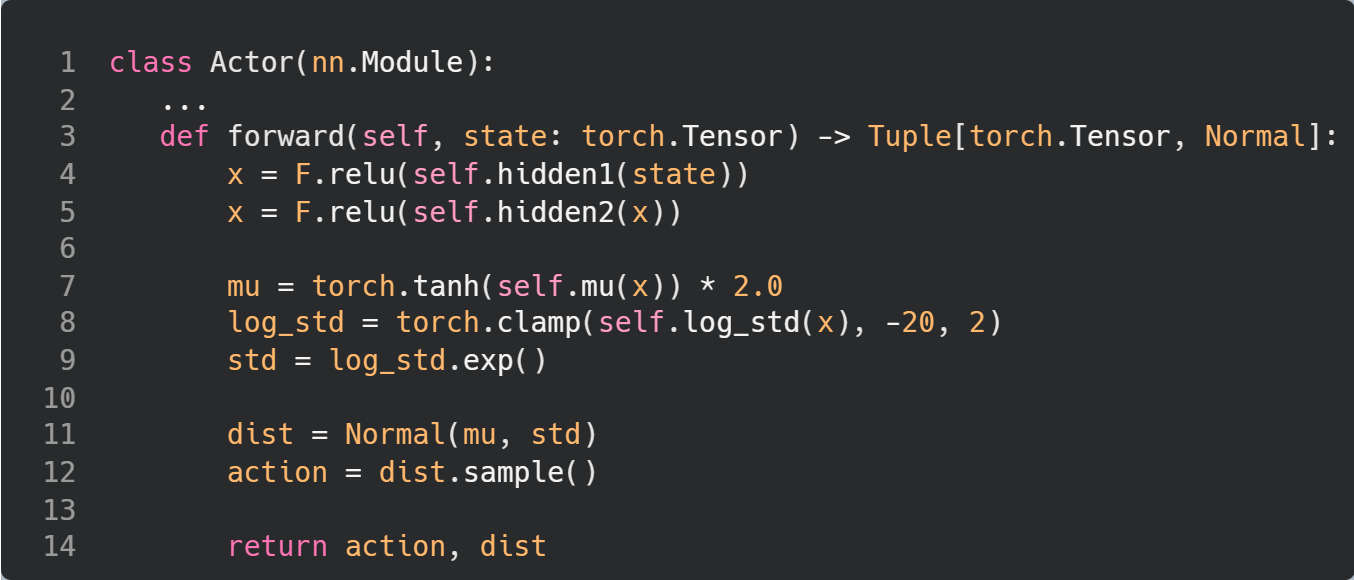
\includegraphics[width=1\linewidth]{assets/impl-actor.png}
  \label{fig:impl_actor}
  \vspace{-0.8em}
\end{figure}
During model updating in \verb|update_model()|, we compute the
bootstrapped target and critic value loss, and then update the
critic network:
\begin{figure}[H]
  \vspace{-0.6em}
  \centering
  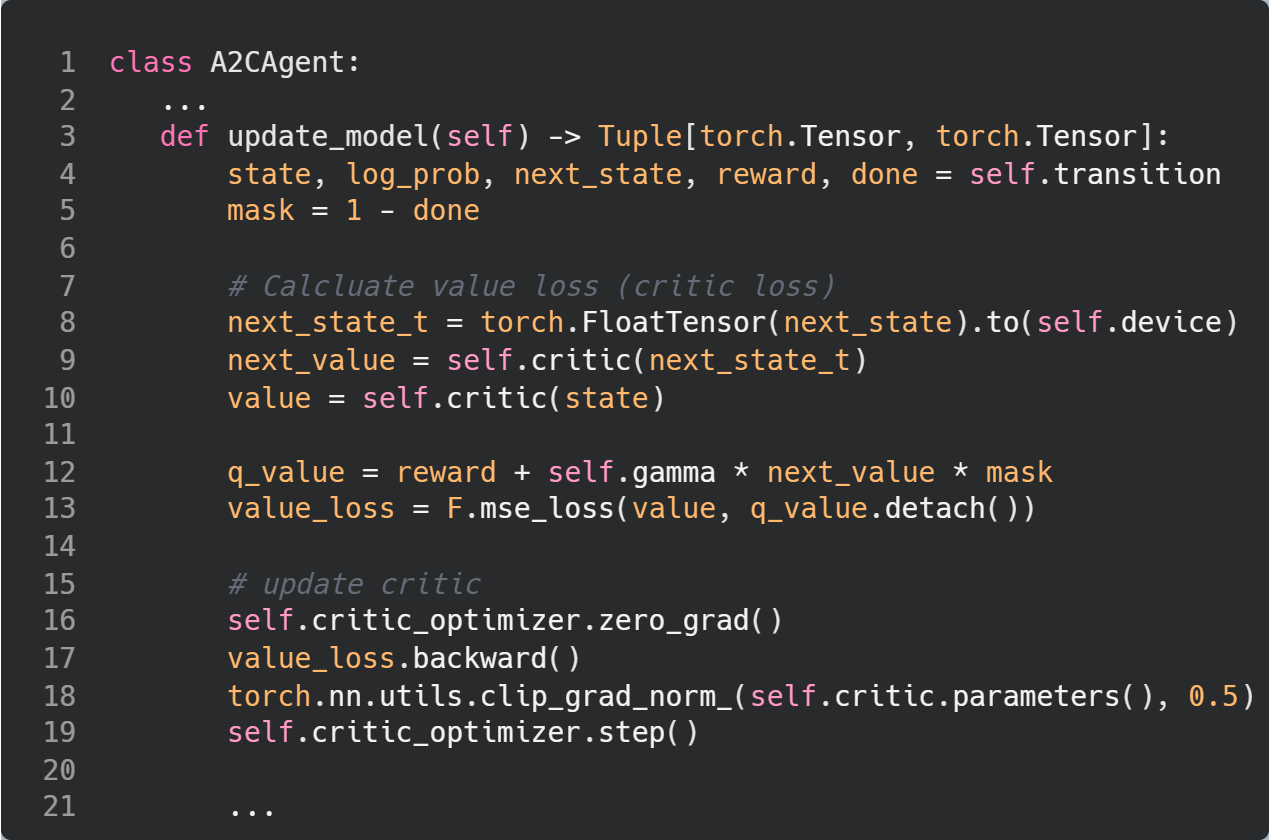
\includegraphics[width=1\linewidth]{assets/impl-update-critic.png}
  \label{fig:impl_update_critic}
  \vspace{-2em}
\end{figure}
The advantage $\delta_t$ is then computed by \verb|q_value| and
\verb|value|, and the policy gradient is updated via backpropagation
using the policy loss (negative objective) with entropy regularization:
\begin{figure}[H]
  \vspace{-0.6em}
  \centering
  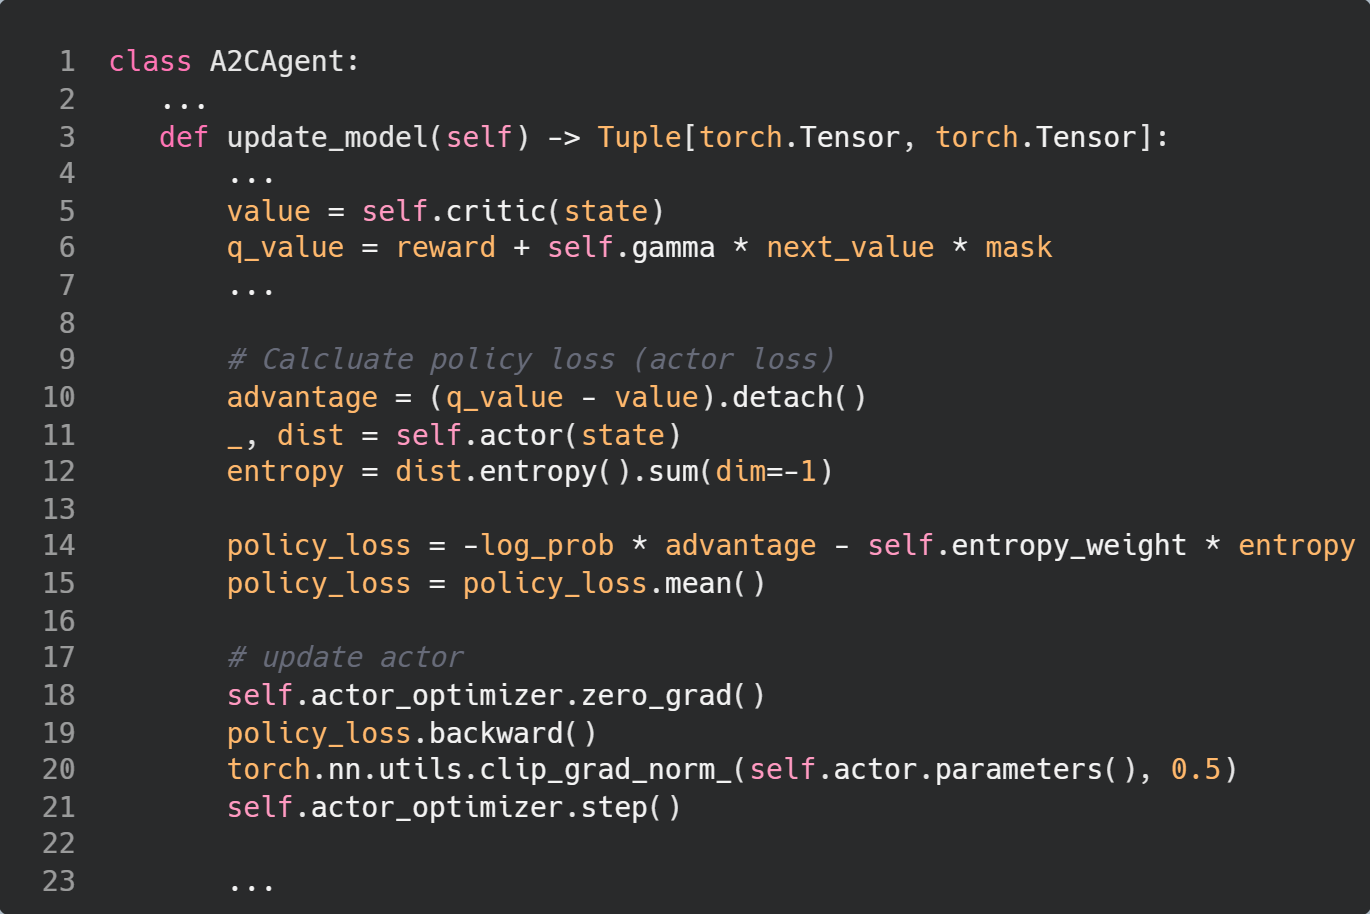
\includegraphics[width=1\linewidth]{assets/impl-update-actor.png}
  \label{fig:impl_update_actor}
  \vspace{-2em}
\end{figure}
Both Actor and Critic networks undergo gradient norm clipping to
$0.5$ before stepping their respective Adam optimizers to maintain
stability.

\subsection{Clipped Surrogate Objective in PPO}
\label{subsec:impl_ppo_clip}

\paragraph{Mathematical Concepts:}
Standard policy gradient algorithms are prone to destructively large
policy updates. PPO resolves this by using a clipped surrogate objective
that constrains the policy update step size. PPO defines the probability
ratio $\rho_t(\theta)$ between the new and old policy:
\begin{equation}
  \rho_t(\theta) = \frac{\pi_\theta(a_t | s_t)}{\pi_{\theta_{\text{old}}}(a_t | s_t)}
  \label{eq:ratio}
\end{equation}
The clipped surrogate objective $L_{\text{CLIP}}(\theta)$ is defined as:
\begin{equation}
  L_{\text{CLIP}}(\theta) = \mathbb{E}_t \left[ \min \left( \rho_t(\theta) \hat{A}_t, \text{clip}(\rho_t(\theta), 1-\epsilon, 1+\epsilon) \hat{A}_t \right) \right]
  \label{eq:ppo_clip}
\end{equation}
where $\epsilon$ is the clipping parameter. The minimum operator takes
the lower bound of the clipped and unclipped objective, which prevents the
policy from driving the ratio $\rho_t$ too far in a direction that
exceedingly improves the objective, while allowing the objective to drop
if the change is detrimental.

\paragraph{Code Implementation:}
In \texttt{ppo\_pendulum-3.py} and \texttt{ppo\_walker-3.py}, the PPO
clipped surrogate objective is computed inside the mini-batch training loop
over the rollout buffer. We evaluate the new probability density and compute
the ratio and clipped actor loss as:
\begin{figure}[H]
  \vspace{-0.6em}
  \centering
  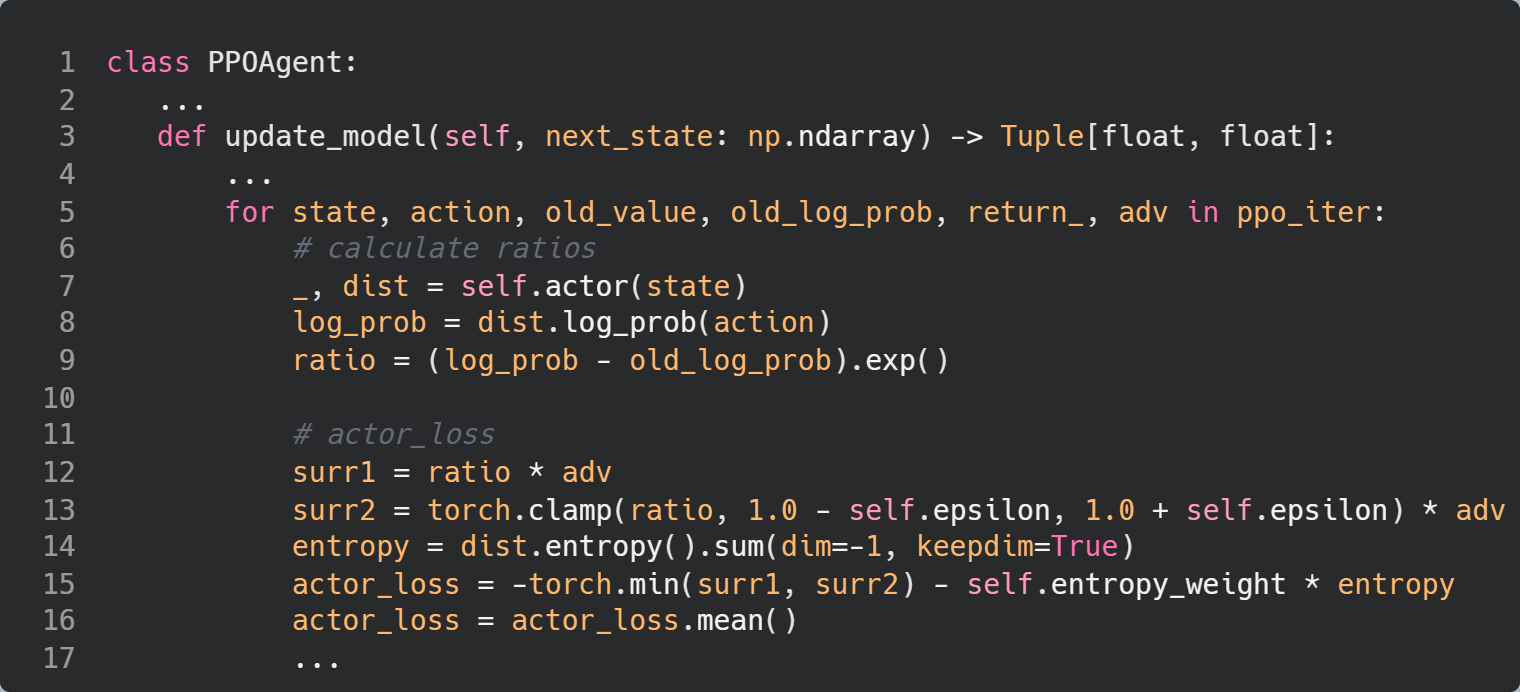
\includegraphics[width=1\linewidth]{assets/impl-ppo-clipped-obj.png}
  \label{fig:impl_ppo_clip}
  \vspace{-2em}
\end{figure}
This objective is minimized (using the negative sign) to maximize the PPO
objective while encouraging policy entropy.

\subsection{Generalized Advantage Estimation (GAE)}
\label{subsec:impl_gae}

\paragraph{Mathematical Concepts:}
GAE addresses the bias-variance trade-off in advantage estimation. GAE scales
between the high-bias TD(0) advantage ($\tau = 0$) and the high-variance Monte
Carlo advantage ($\tau = 1$) via an exponential discount factor $\tau \in [0, 1]$.
The GAE advantage estimator $\hat{A}^{\text{GAE}}_t$ is given by:
\begin{equation}
  \hat{A}^{\text{GAE}}_t = \sum_{l=0}^{\infty} (\gamma \tau)^l \delta^V_{t+l}
  \label{eq:gae_inf}
\end{equation}
where $\delta^V_t = r_t + \gamma V_\phi(s_{t+1}) (1 - d_t) - V_\phi(s_t)$ is the TD
residual, and $(1 - d_t)$ is the environment termination/truncation flag.
The estimator is calculated recursively in reverse starting from
the end of the trajectory:
\begin{equation}
  \hat{A}^{\text{GAE}}_t = \delta^V_t + \gamma \tau (1 - d_t) \hat{A}^{\text{GAE}}_{t+1}
  \label{eq:gae_recur}
\end{equation}
The regression target for training the state-value function $V_\phi$ is then
computed as the sum of the estimated advantage and the current state value:
\begin{equation}
  R_t = \hat{A}^{\text{GAE}}_t + V_\phi(s_t)
  \label{eq:value_target}
\end{equation}

\paragraph{Code Implementation:}
The recursive GAE is implemented in the \verb|compute_gae()|.
It starts from the end of the rollout buffers and moves backward in time:
\begin{figure}[H]
  \vspace{-0.6em}
  \centering
  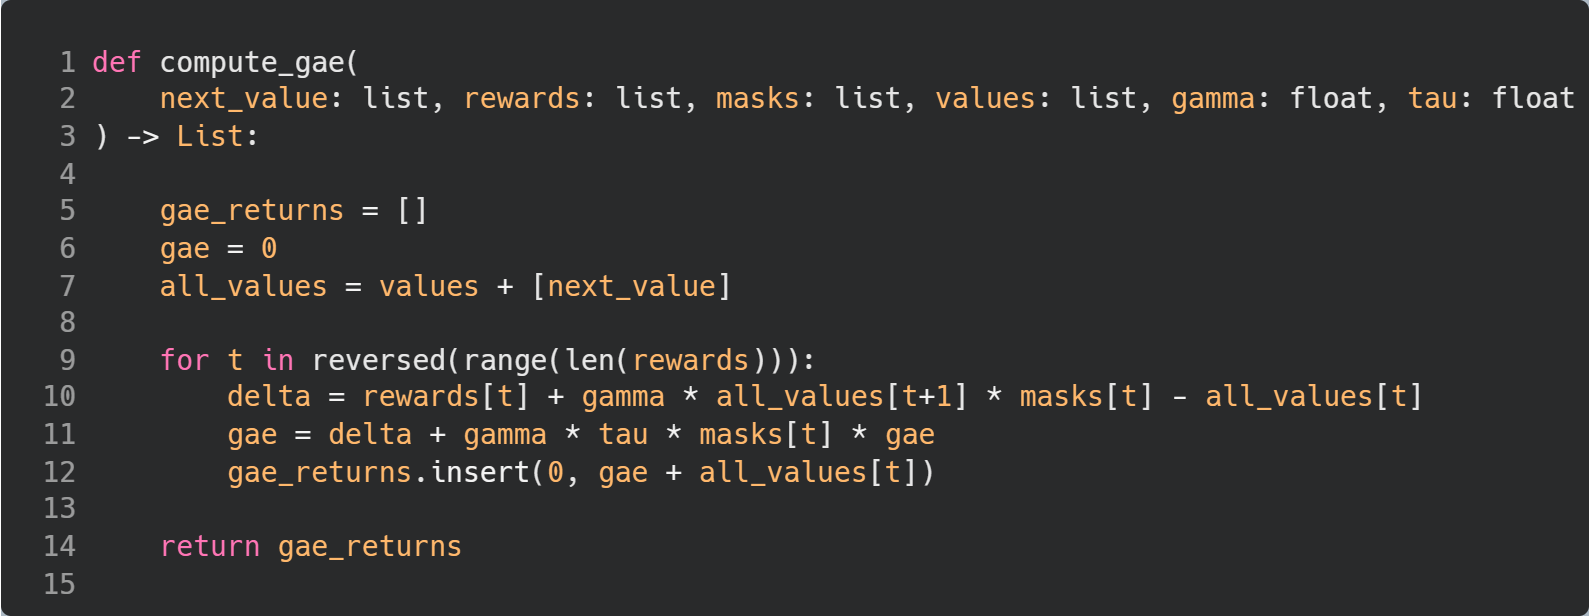
\includegraphics[width=1\linewidth]{assets/impl-gae.png}
  \label{fig:impl_gae}
  \vspace{-2em}
\end{figure}
Here, \texttt{masks[t]} represents $(1 - d_t)$ to zero out the bootstrap
when the episode terminates. The returned list contains the target returns
$R_t$ used to optimize the Critic's network parameters via MSE loss:
\begin{figure}[H]
  \vspace{-0.6em}
  \centering
  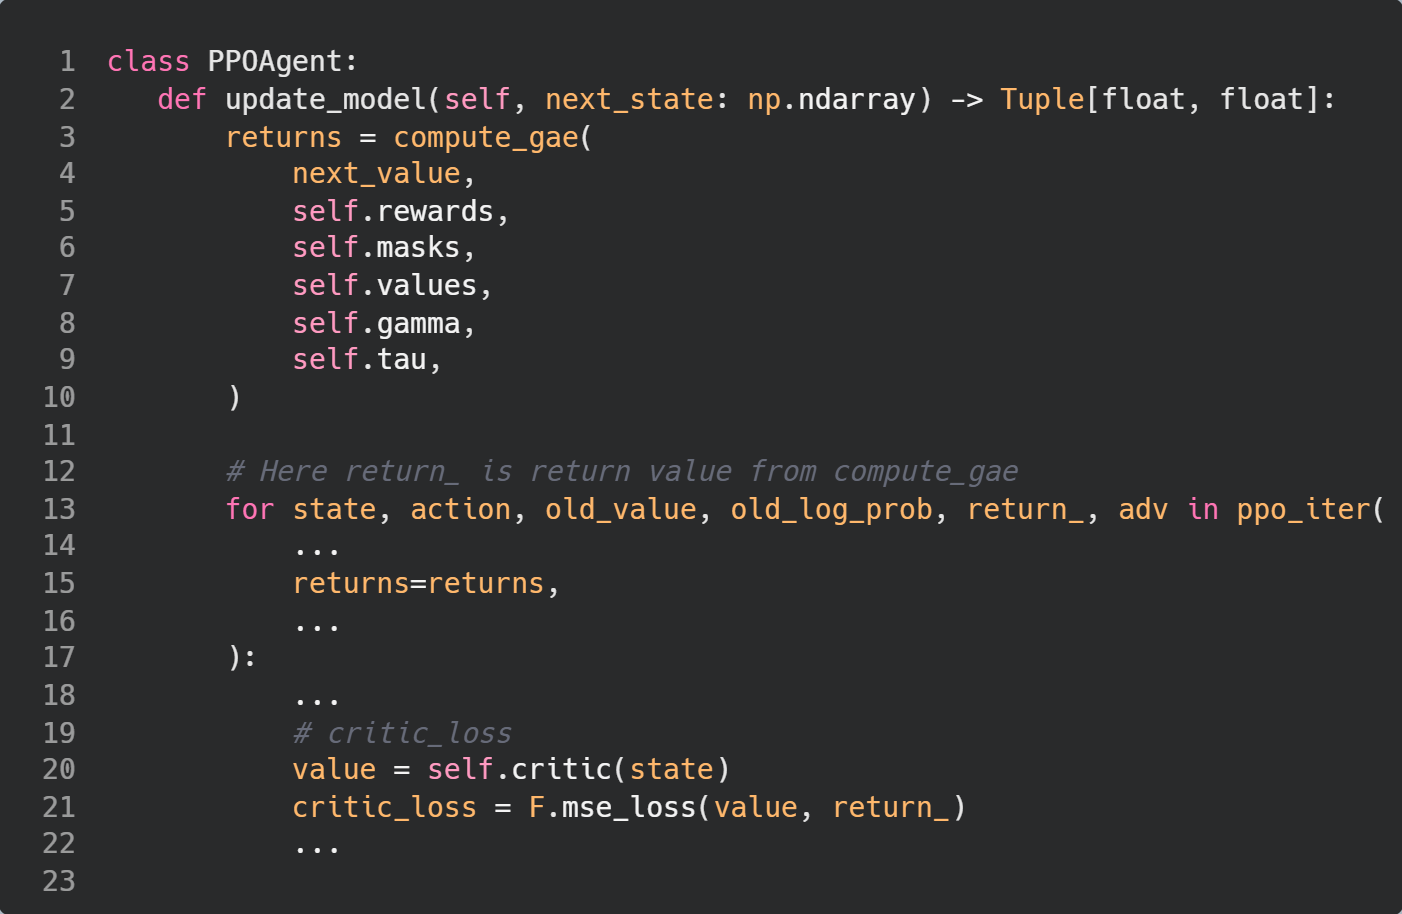
\includegraphics[width=1\linewidth]{assets/impl-gae-update-critic.png}
  \label{fig:impl_gae_update_critic}
  \vspace{-2em}
\end{figure}

\subsection{Environment Sample Collection}
\label{subsec:impl_samples}

A2C and PPO employ fundamentally different sample collection styles:
\begin{itemize}[itemsep=-3pt]
  \item \textbf{A2C (Online, Single-Step)}: Samples a single transition $[s_t, a_t, s_{t+1}, r_t, d_t]$, immediately updates both the Actor and Critic networks, and discards the transition.
  \item \textbf{PPO (Batch, Rollout Buffer)}: Collects a long trajectory of environment steps ($T = 2000$ or $2048$) in buffers, recursively computes advantages/returns, and updates the models over multiple epochs via randomized mini-batches.
\end{itemize}
\begin{figure}[H]
  \vspace{-0.6em}
  \centering
  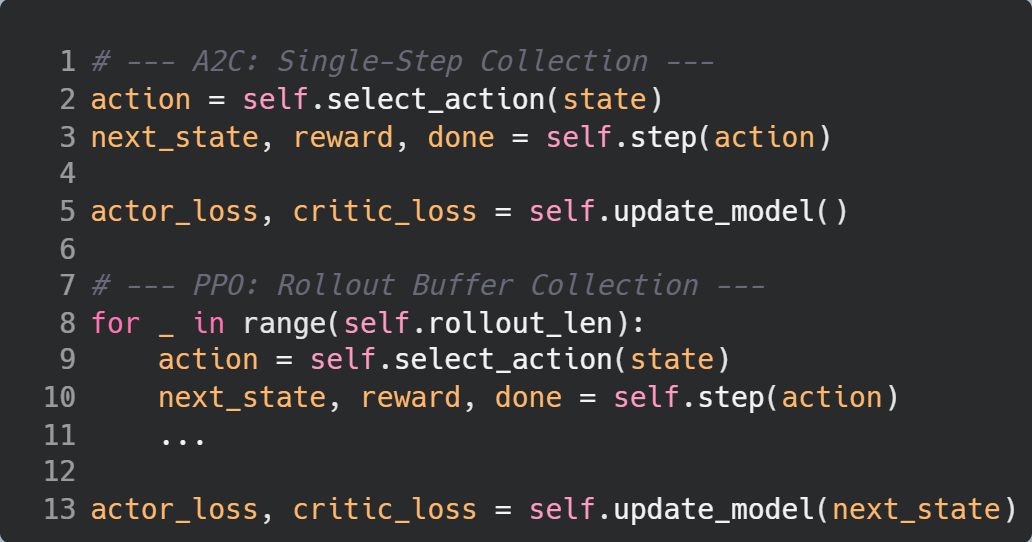
\includegraphics[width=1\linewidth]{assets/impl-sample-collect.png}
  \label{fig:impl_sample_collect}
  \vspace{-2em}
\end{figure}
In PPO, \verb|select_action()| and \verb|step()| collect the trajectory. 
After collecting a full trajectory, \verb|update_model()| will update the models
multiple times via generator \verb|ppo_iter()|.

\subsection{Exploration Strategy in On-Policy RL}
\label{subsec:impl_exploration}

In this lab, since both A2C and PPO are on-policy algorithms, they can easily
get stuck in local optima if the policy becomes deterministic too early. To
ensure the agent continues to explore the continuous state-action space, two
key mechanisms are introduced:
\begin{itemize}[itemsep=-3pt]
  \item \textbf{Stochastic Training vs. Deterministic Testing}: During
    training, the Actor network outputs the mean $\mu(s)$ and standard deviation
    $\sigma(s)$ of a Gaussian distribution. Actions are sampled from the
    distribution to encourage exploration of the environment. During testing
    (\verb|self.is_test = True|), the agent deterministically selects the mean
    action (\verb|dist.mean|) to ensure stable and optimal evaluation performance.
  \item \textbf{Entropy Penalty in Actor Loss}: To prevent the action standard
    deviation $\sigma(s)$ from collapsing to zero too quickly, an entropy
    regularization term is added to the Actor's loss function. Because the
    entropy of a Gaussian distribution increases with its variance, minimizing
    this negative term penalizes the network for shrinking standard deviations,
    successfully maintaining a healthy amount of exploration.
\end{itemize}

\subsection{Weights \& Biases (W\&B) Model Performance Tracking}
\label{subsec:impl_wandb}

I integrated \textbf{Weights \& Biases (W\&B)} into our codebase to monitor model
convergence, learning dynamics, and performance metrics in real-time. To
ensure accurate comparative analysis, the x-axis for all logs is explicitly bound
to the environment interaction step using \verb|wandb.define_metric("step")|
and aligning all logged parameters to it:
\begin{itemize}[itemsep=-3pt]
  \item \textbf{Actor Loss}: Shows the progress of policy optimization. In PPO,
  this reflects the clipped surrogate loss; in A2C, it shows the stochastic
  policy gradient loss.
  \item \textbf{Critic Loss}: Evaluates state-value estimation performance (MSE
  loss of $V(s)$ relative to bootstrapped/GAE returns).
  \item \textbf{Return / Eval Return}: Tracks the raw training return of each
  completed episode and the average evaluation score over 20 deterministic seed
  evaluations (run every \verb|eval_interval| episodes).
\end{itemize}

\subsection{Bonus: Continuous Control Optimization}
\label{sec:bonus}

Scaling PPO to high-dimensional continuous control locomotion like
Walker2d-v5 is notoriously difficult due to large coordinate variances,
complex joint dynamics, and sensitive reward signals. In Task 3
(\verb|ppo_walker-3.py|), I incorporated several continuous control
optimization strategies, which proved absolutely critical in enabling
PPO to solve the environment:

\paragraph{Observation Normalization (\texttt{--obs-norm}):}
Raw state observations in Walker2d can have highly varying scales, which
distort neural network weights and cause unstable gradient directions. I
implemented observation normalization using a running mean and standard
deviation:
\begin{equation}
  s_t^{\text{norm}} = \text{clip}\left(\frac{s_t - \mu_s}{\sqrt{\sigma^2_s + 10^{-8}}}, -10, 10\right)
  \label{eq:obs_norm}
\end{equation}
where $\mu_s$ and $\sigma^2_s$ are updated online using Welford's algorithm
(\texttt{RunningMeanStd}). This normalizes all observation dimensions to
zero-mean and unit variance.
\begin{figure}[H]
  \vspace{-0.6em}
  \centering
  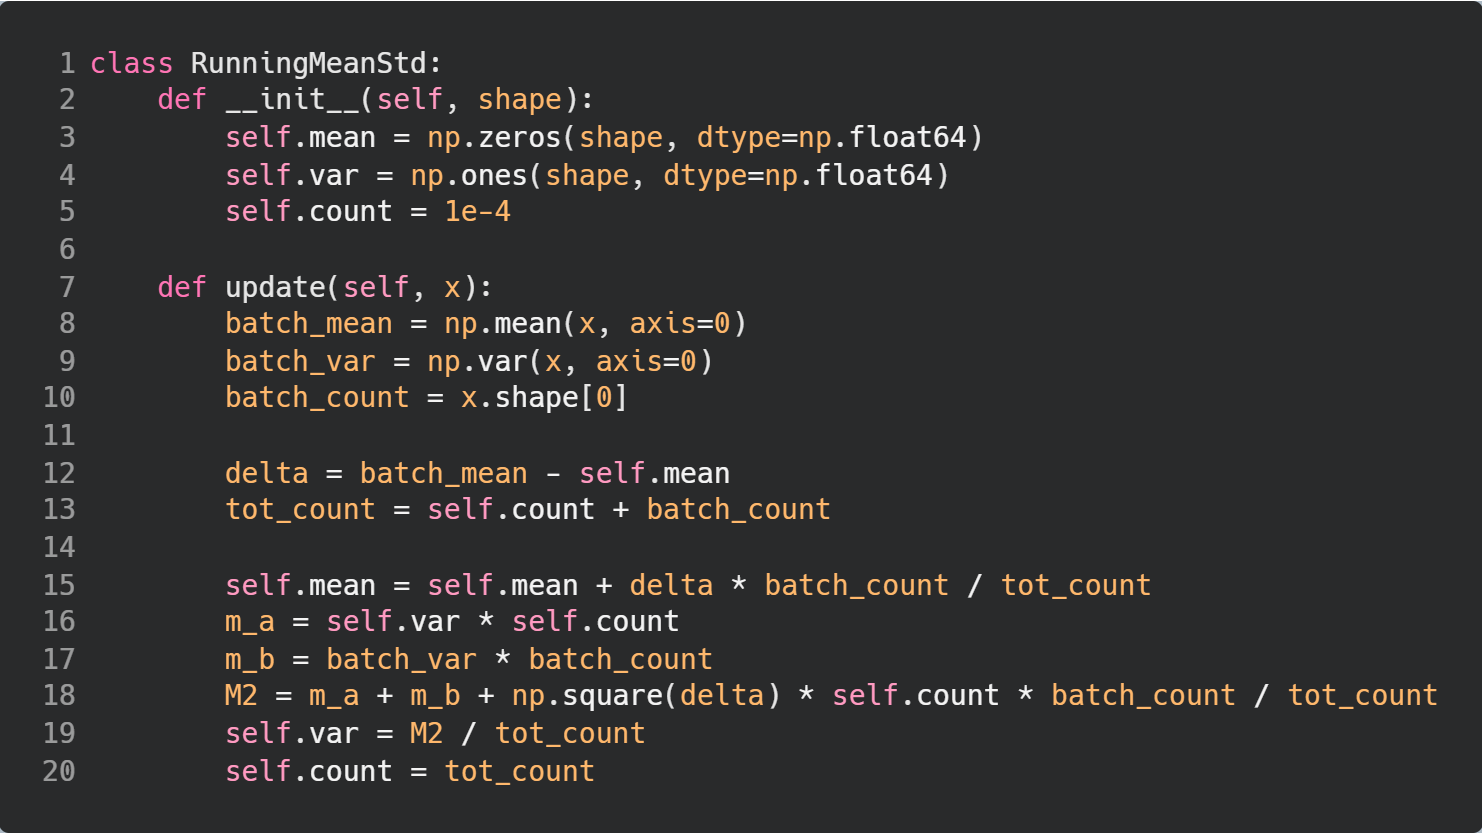
\includegraphics[width=1\linewidth]{assets/impl-rms.png}
  \label{fig:impl_rms}
  \vspace{-2em}
\end{figure}

\paragraph{Advantage Normalization (\texttt{--adv-norm}):}
The advantage values computed over a rollout buffer can vary widely across
iterations, causing huge fluctuations in actor updates. By normalizing the
advantages across each mini-batch:
\begin{equation}
  \hat{A}_t^{\text{norm}} = \frac{\hat{A}_t - \mu_A}{\sigma_A + 10^{-8}}
  \label{eq:adv_norm}
\end{equation}
we force the advantage distribution to zero-mean and unit variance, keeping
policy gradient updates exceptionally stable.

\paragraph{Learning Rate Cosine Scheduling (\texttt{--sched}):}
Using a fixed learning rate throughout training often leads to late-stage
policy oscillations and prevents convergence to high-precision walking gaits.
I integrated a Cosine Annealing learning rate schedule. Gradually annealing
the learning rate allows PPO to make large, fast progress early on, and
smoothly decay to precise, micro-level adjustments as the agent reaches
the optimal gait.

\section{Analysis and Discussions}
\label{sec:analysis}

\subsection{Training Curves}
\label{subsec:analysis_curves}

The training curves represent the evaluation score, averaging across 20
test seeds, plotted against the total number of environment steps.

\textbf{Task 1: A2C on Pendulum-v1}. As shown in \cref{fig:task1_curve},
A2C exhibits extremely high variance and slow convergence. Achieve around
-150 at 120k steps, but quickly drop at 150k steps.

\textbf{Task 2: PPO on Pendulum-v1}. In \cref{fig:task2_curve}, PPO
exhibits more stable performance, reaching score -200 in just 30k steps.

\textbf{Task 3: PPO on Walker2d-v5}. In \cref{fig:task3_curve}, Benefiting
from continuous control optimizations,
Walker2d-v5 achieves steady growth, surpassing an average return of 2500
within 1M steps. And finally Achieves 4000 score around 2M steps.

\begin{figure}[H]
  \centering
  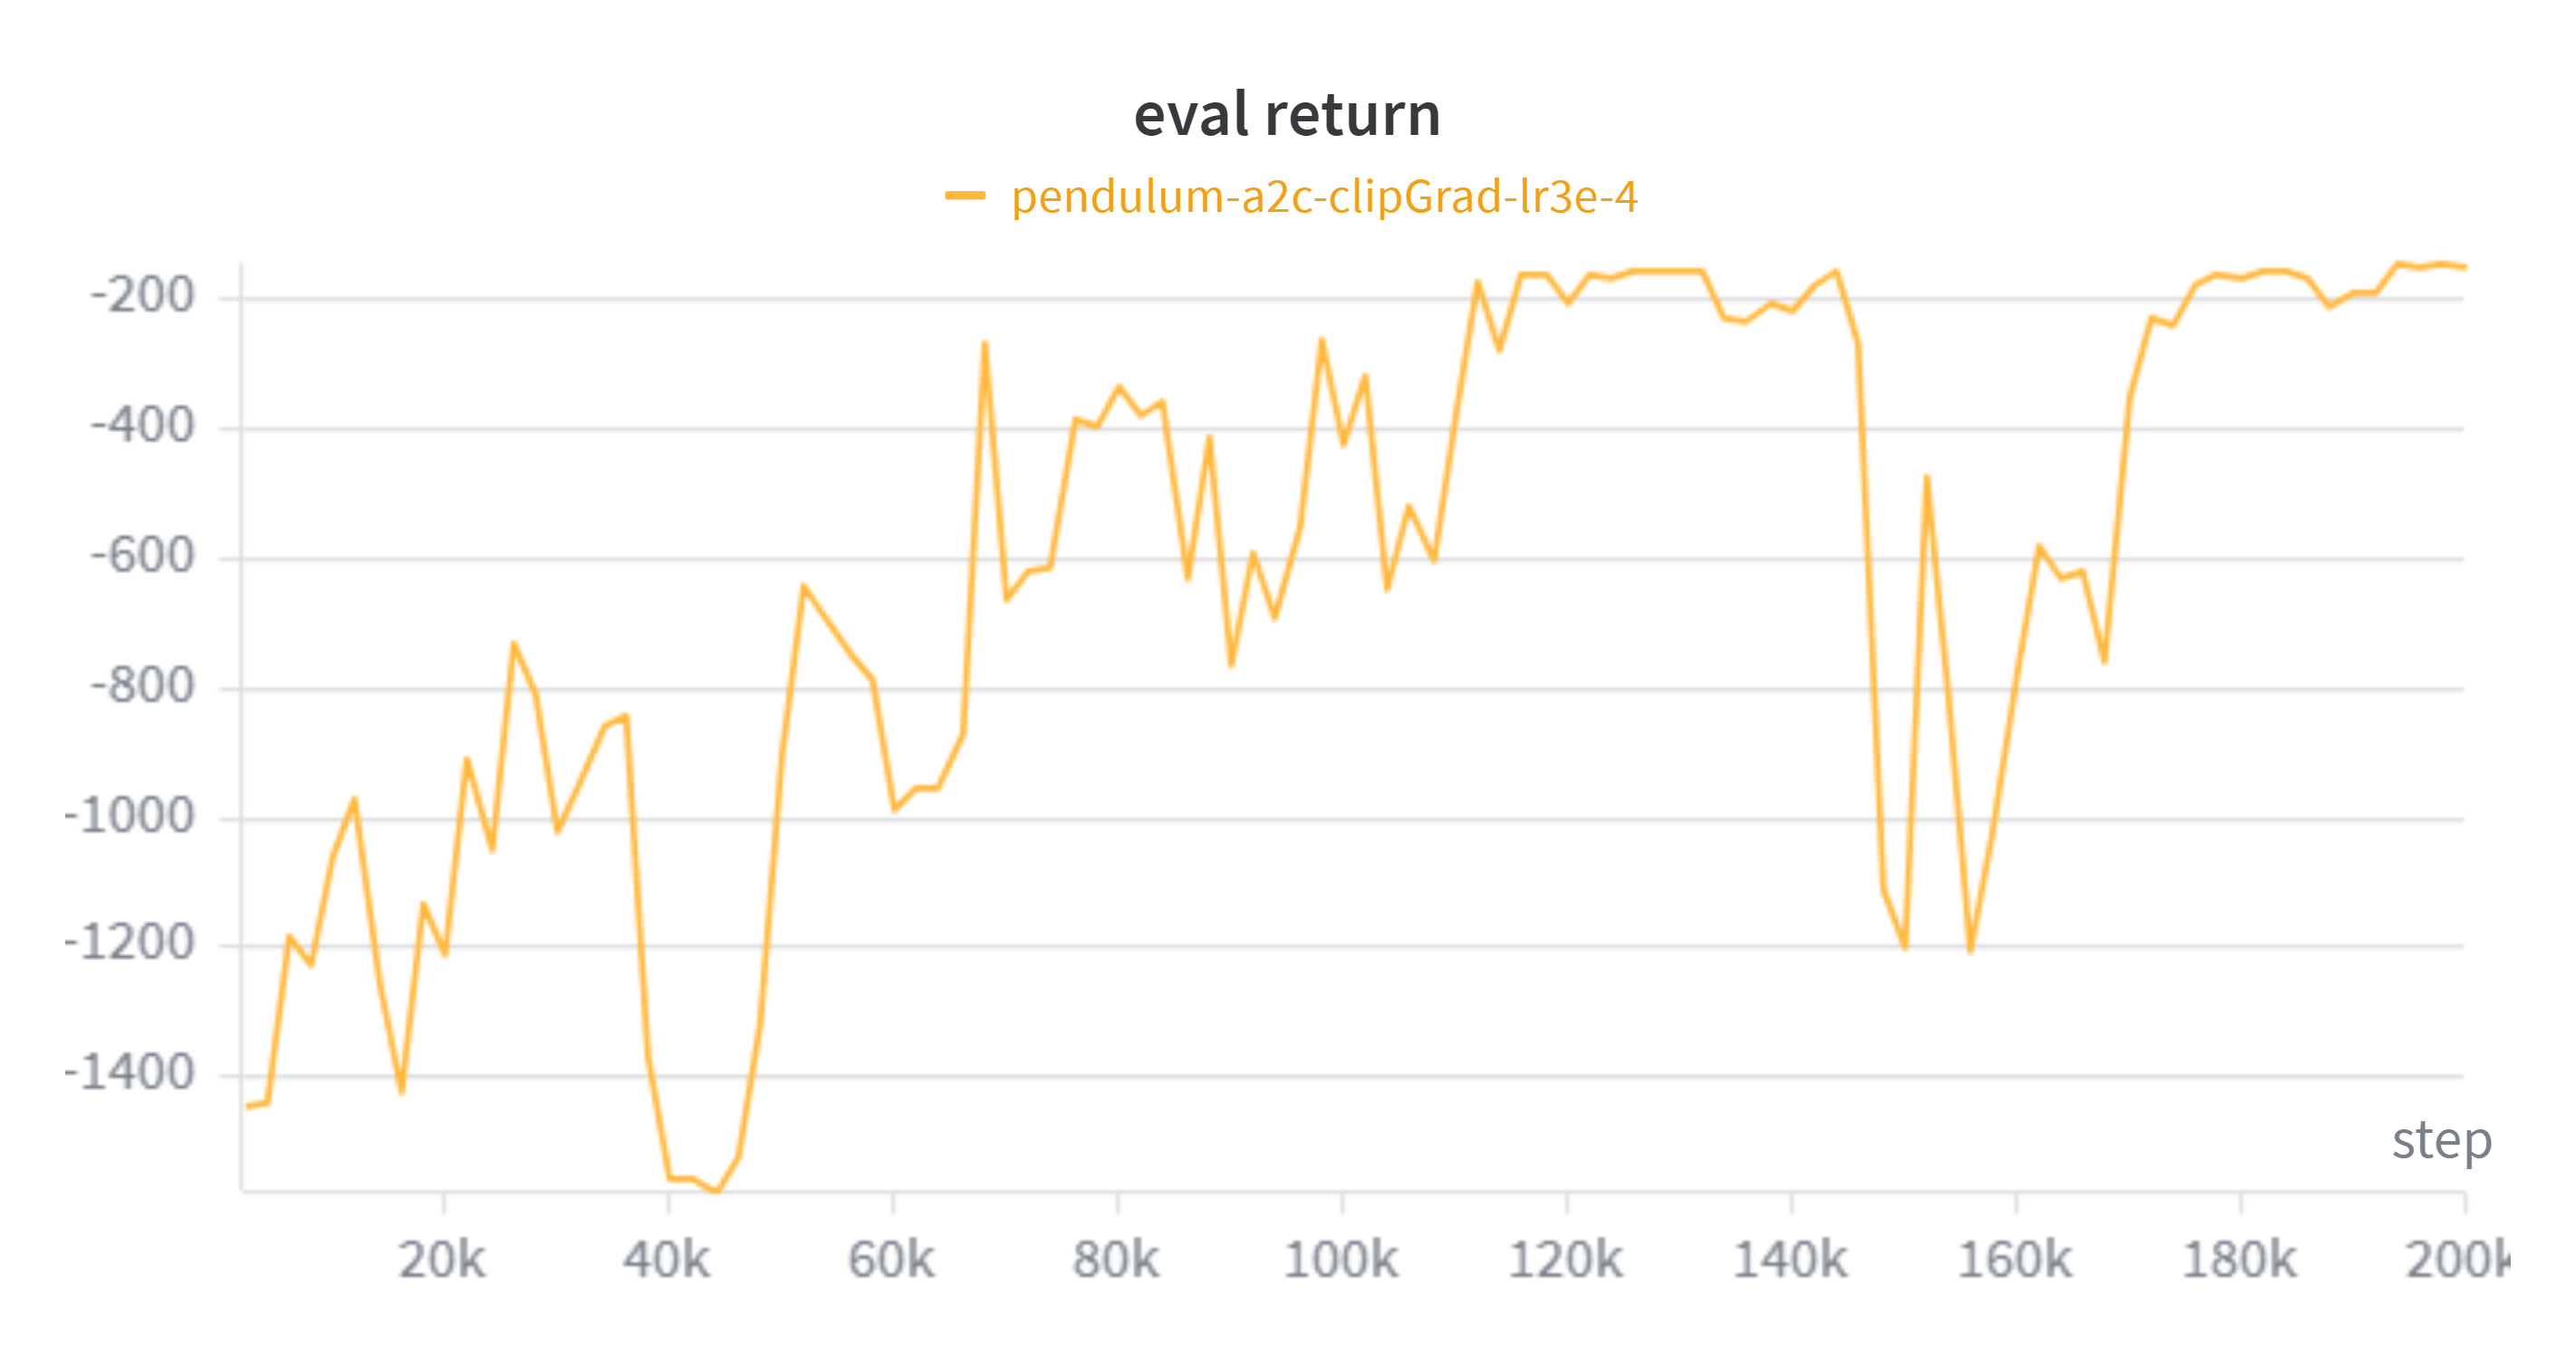
\includegraphics[width=0.9\linewidth]{assets/task1_curve.png}
  \caption{\textbf{Task 1 A2C Pendulum-v1} training curve.}
  \label{fig:task1_curve}
\end{figure}

\begin{figure}[H]
  \centering
  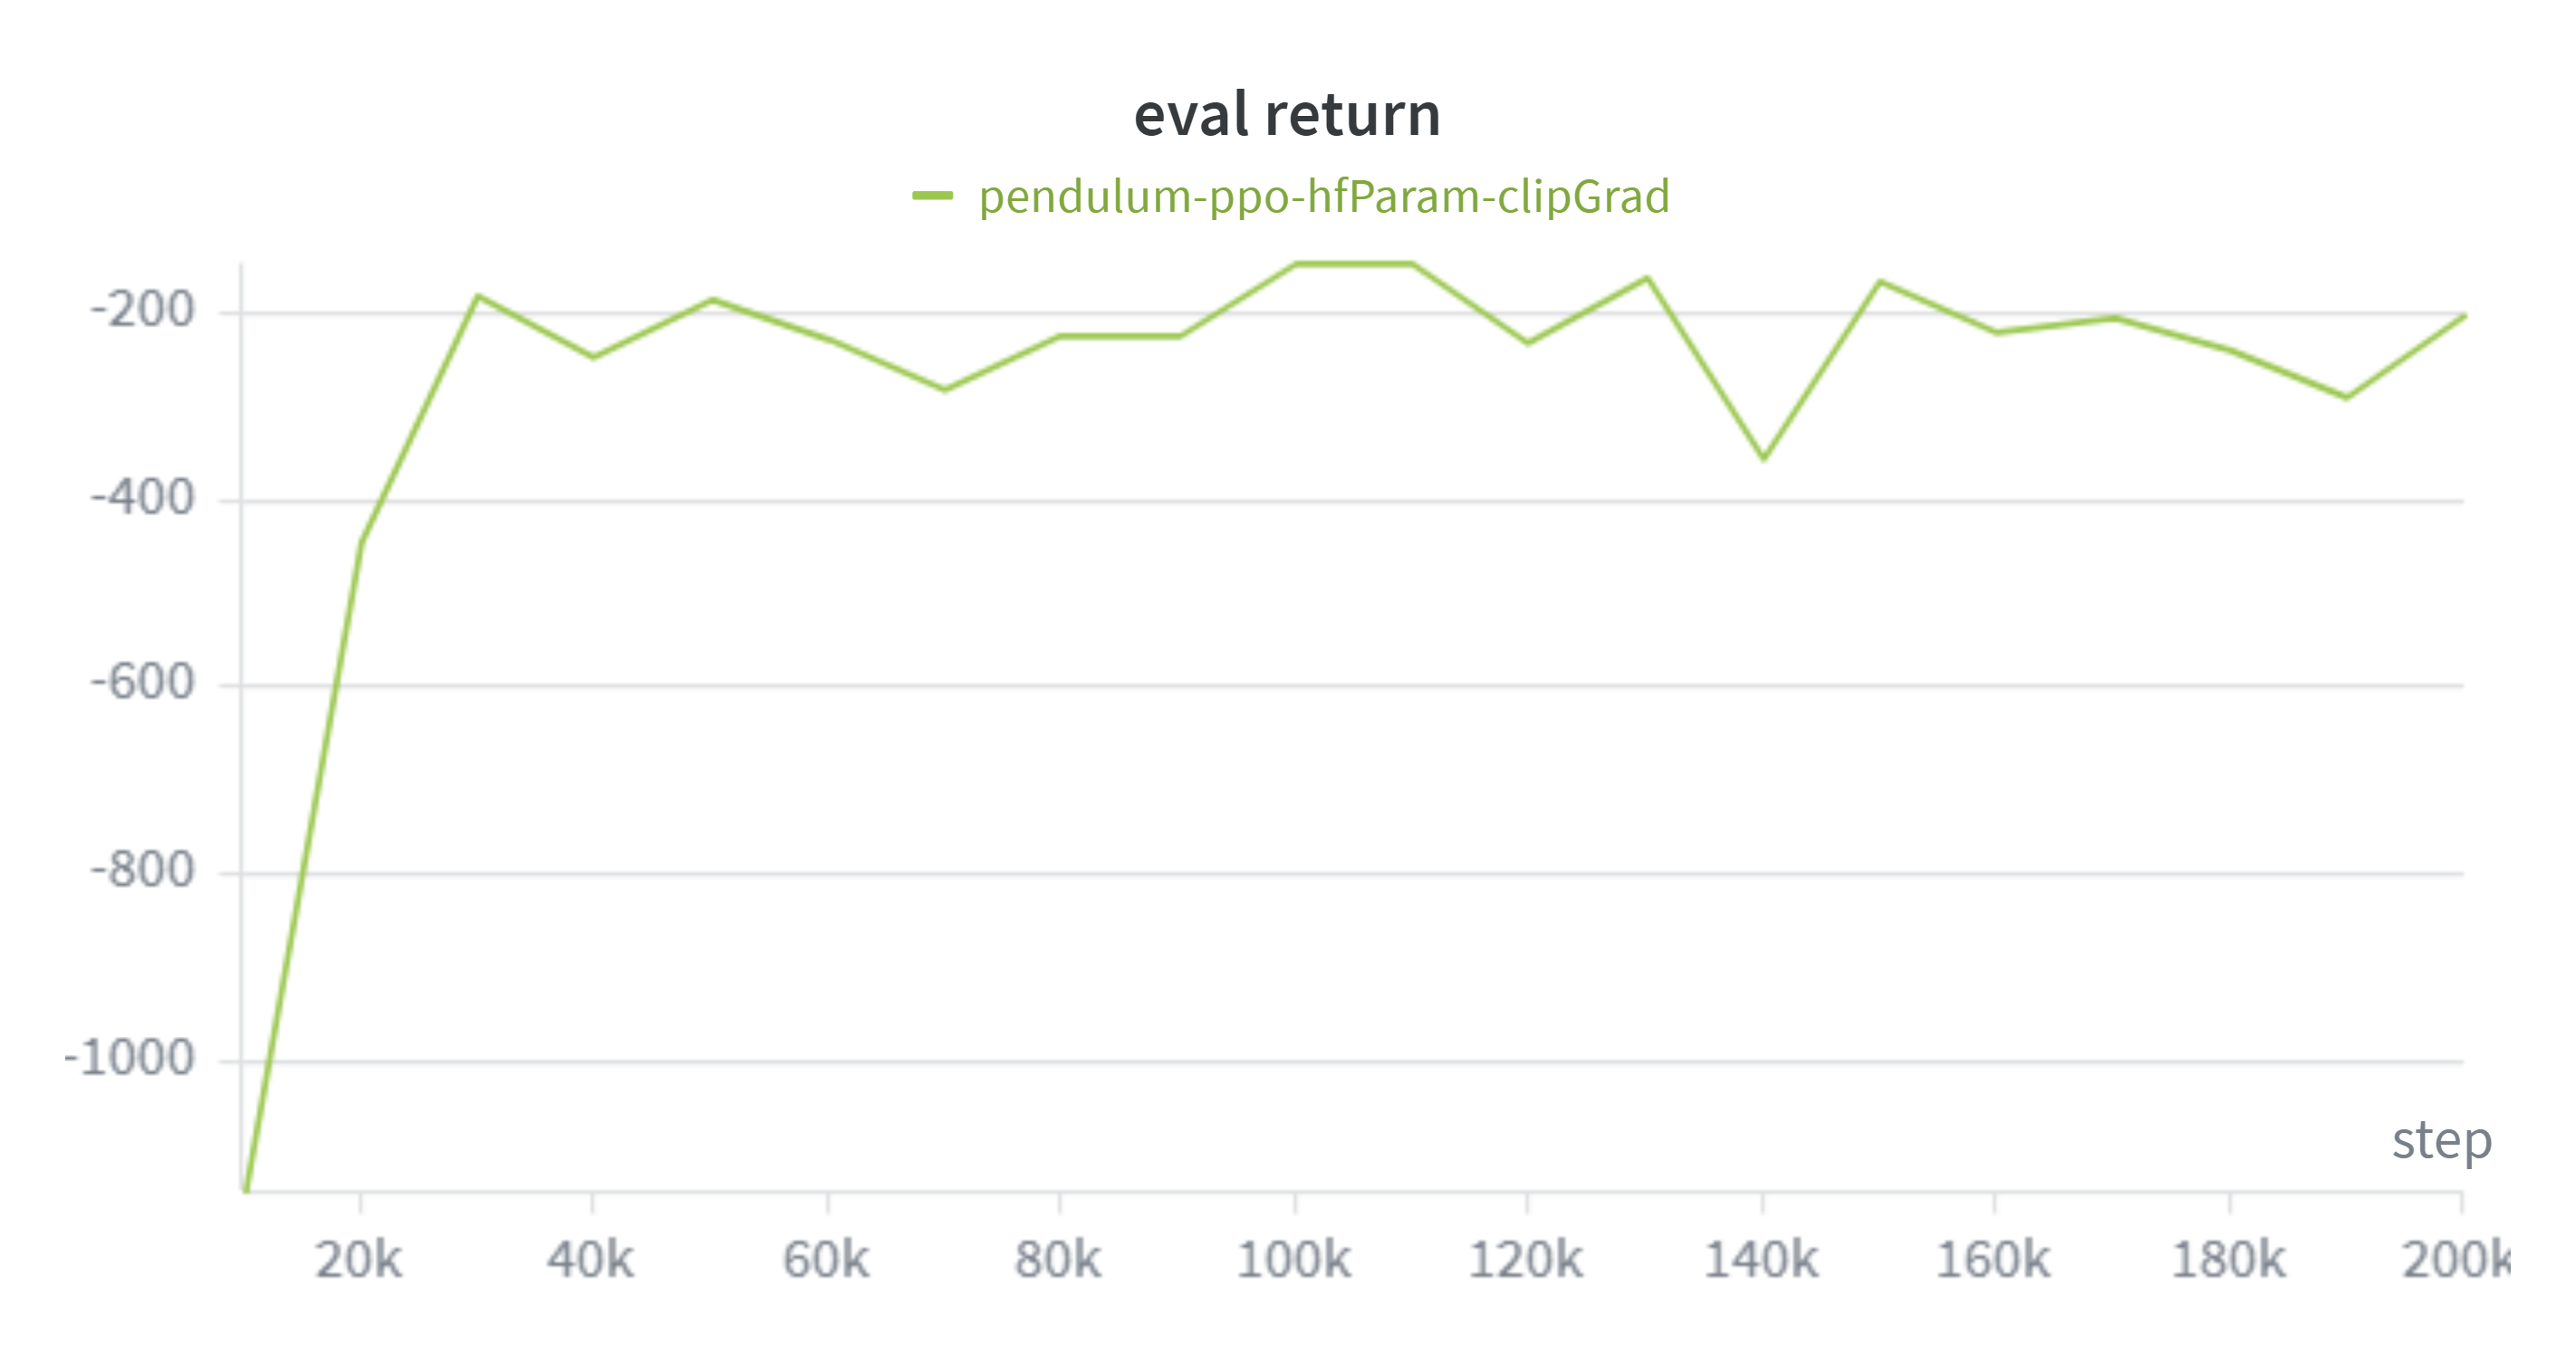
\includegraphics[width=0.9\linewidth]{assets/task2_curve.png}
  \caption{\textbf{Task 2 PPO Pendulum-v1} training curve.}
  \label{fig:task2_curve}
\end{figure}

\begin{figure}[H]
  \centering
  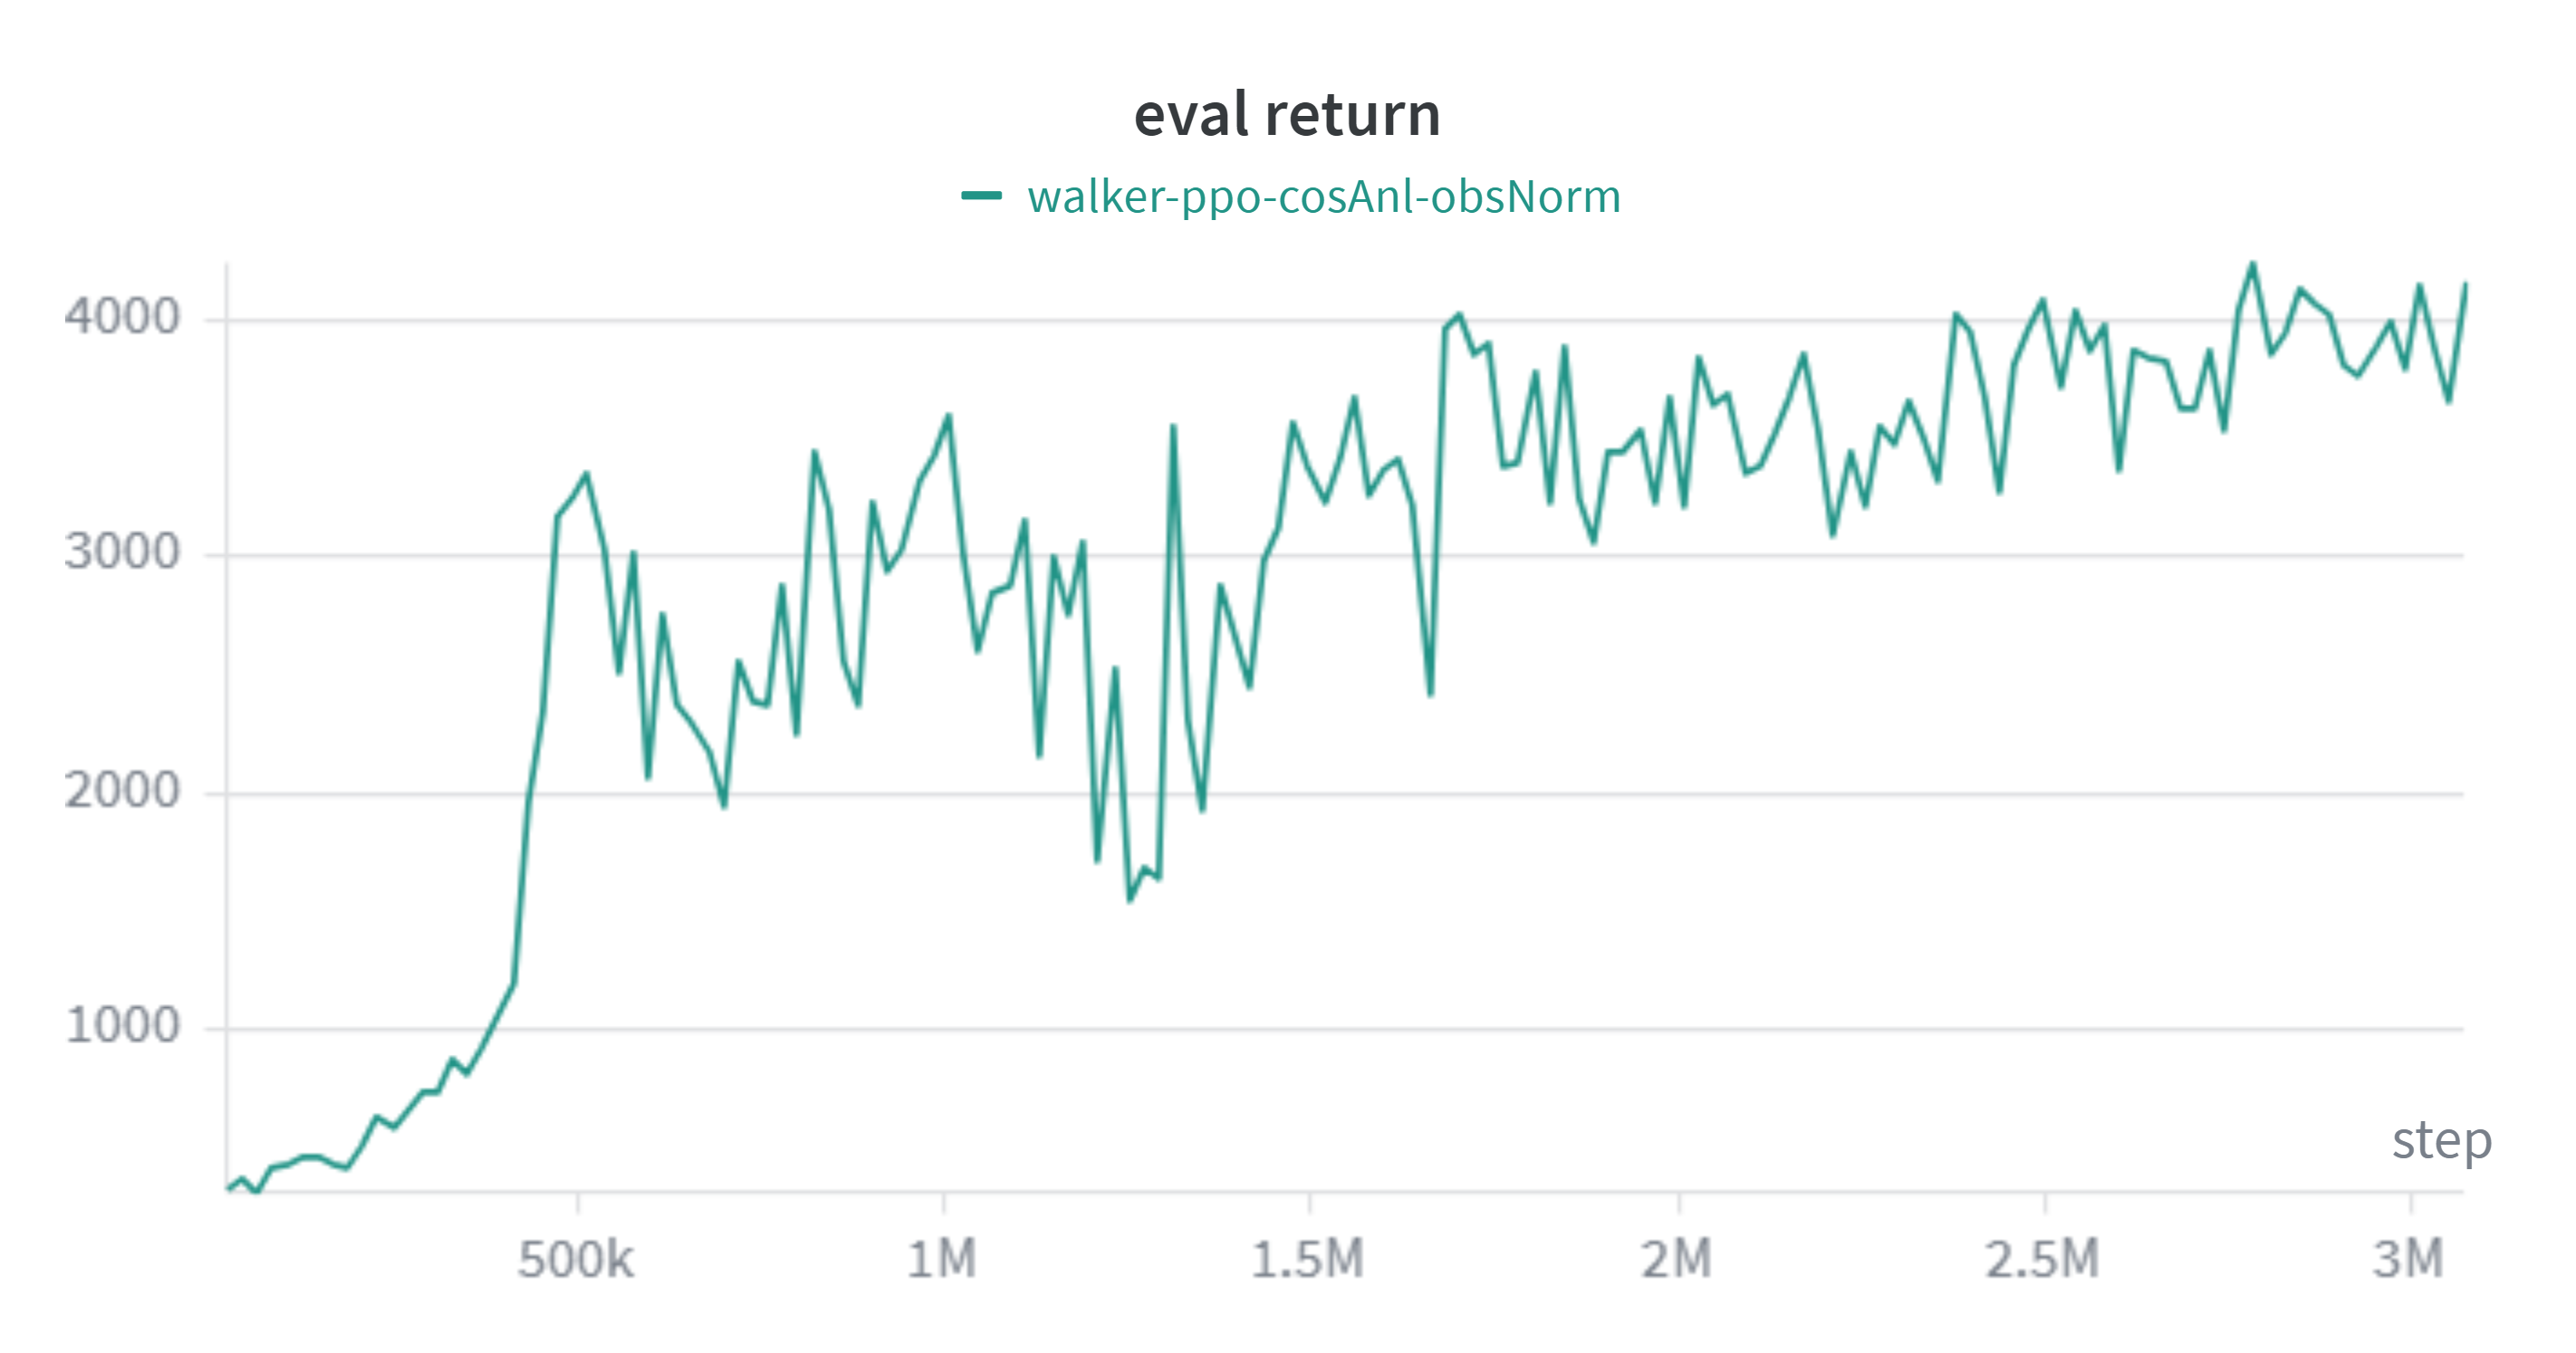
\includegraphics[width=0.9\linewidth]{assets/task3_curve.png}
  \caption{\textbf{Task 3 PPO Walker2d-v5} training curve.}
  \label{fig:task3_curve}
\end{figure}

\subsection{Evaluation Results}
\label{subsec:analysis_eval}

The screenshots of evaluation results are in \cref{fig:task1_eval},
\cref{fig:task2_eval}, and \cref{fig:task3_eval}.
\textbf{Task 1 A2C Pendulum-v1} achieve -143.4147 for its best
checkpoint saved in 19.8k steps, while \textbf{Task 2 PPO Pendulum-v1}
achieve -145.9427 in 10k steps. Both Task successfully achieve score
above -150. The scores for \textbf{Task 3 PPO Walker2d-v5} are summarized
in \cref{tab:task3_eval}. Within 1M steps, the model has already
performed over 2500 score.


\begin{figure}[H]
  \centering
  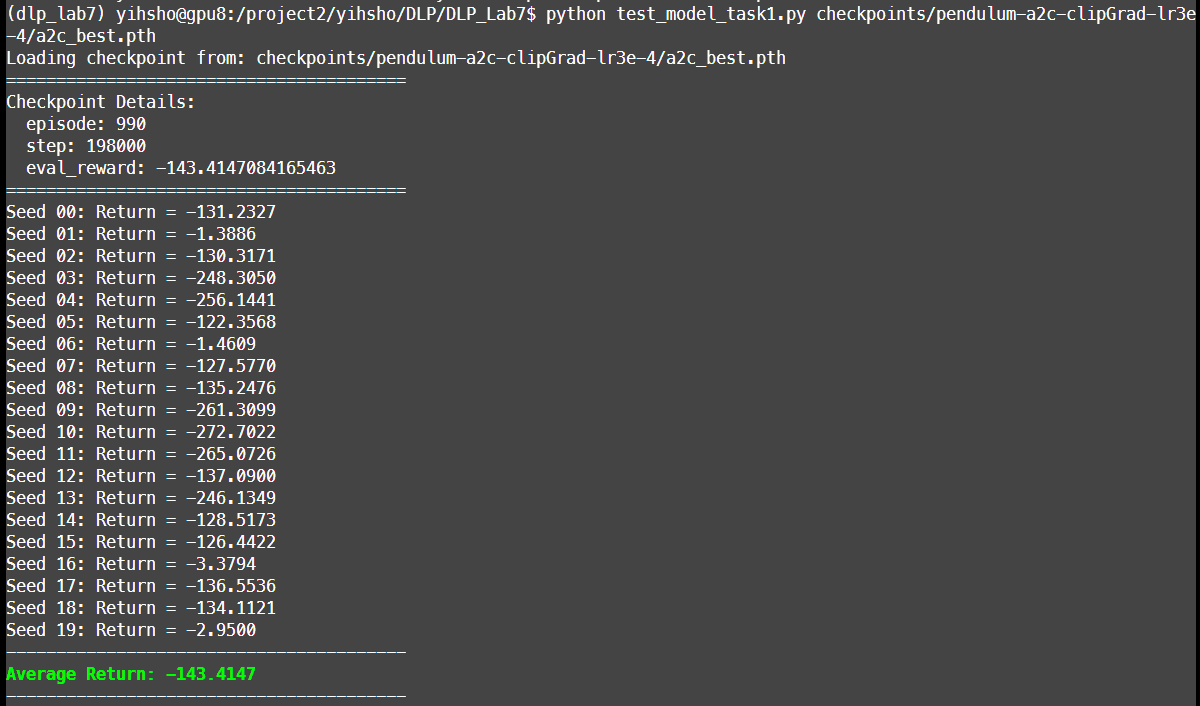
\includegraphics[width=0.9\linewidth]{assets/task1_eval.png}
  \caption{\textbf{A2C Pendulum-v1} evaluation terminal output. The
    checkpoint is selected by highest evaluated score.}
  \label{fig:task1_eval}
\end{figure}

\begin{figure}[H]
  \centering
  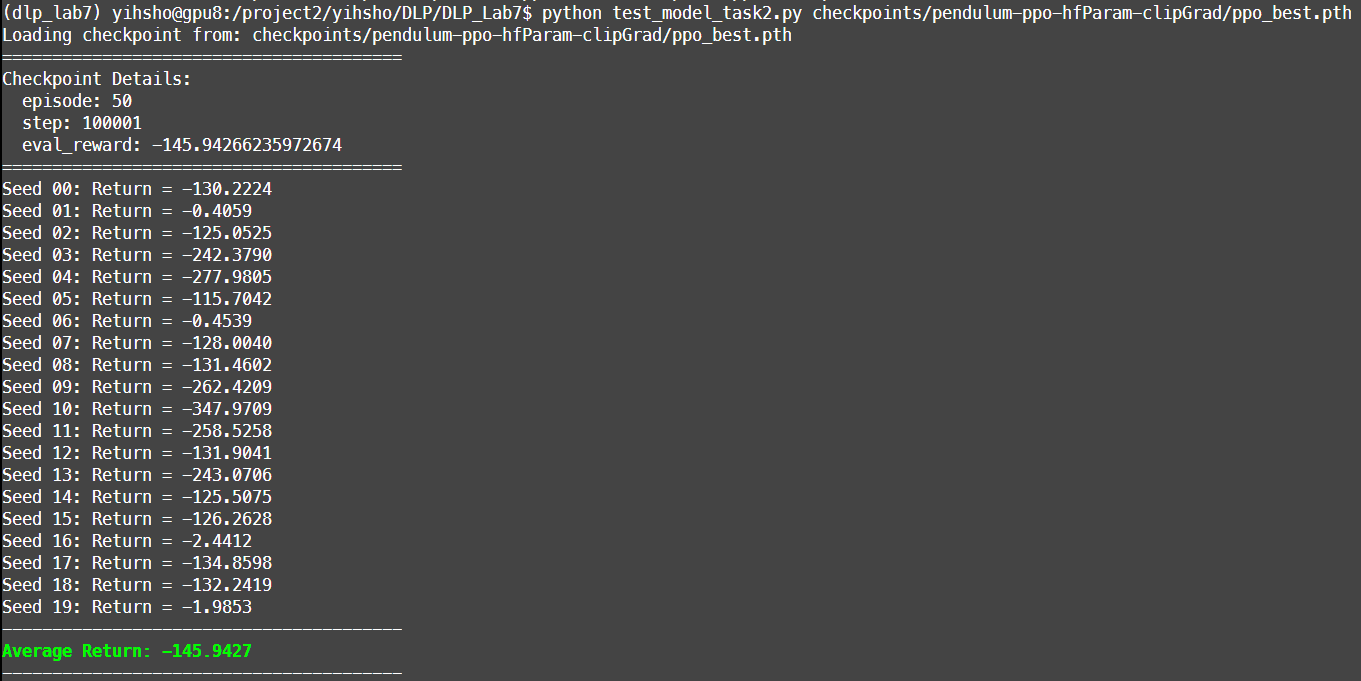
\includegraphics[width=0.9\linewidth]{assets/task2_eval.png}
  \caption{\textbf{PPO Pendulum-v1} evaluation terminal output. The
    checkpoint is selected by highest evaluated score.}
  \label{fig:task2_eval}
\end{figure}

\begin{figure}[H]
  \centering
  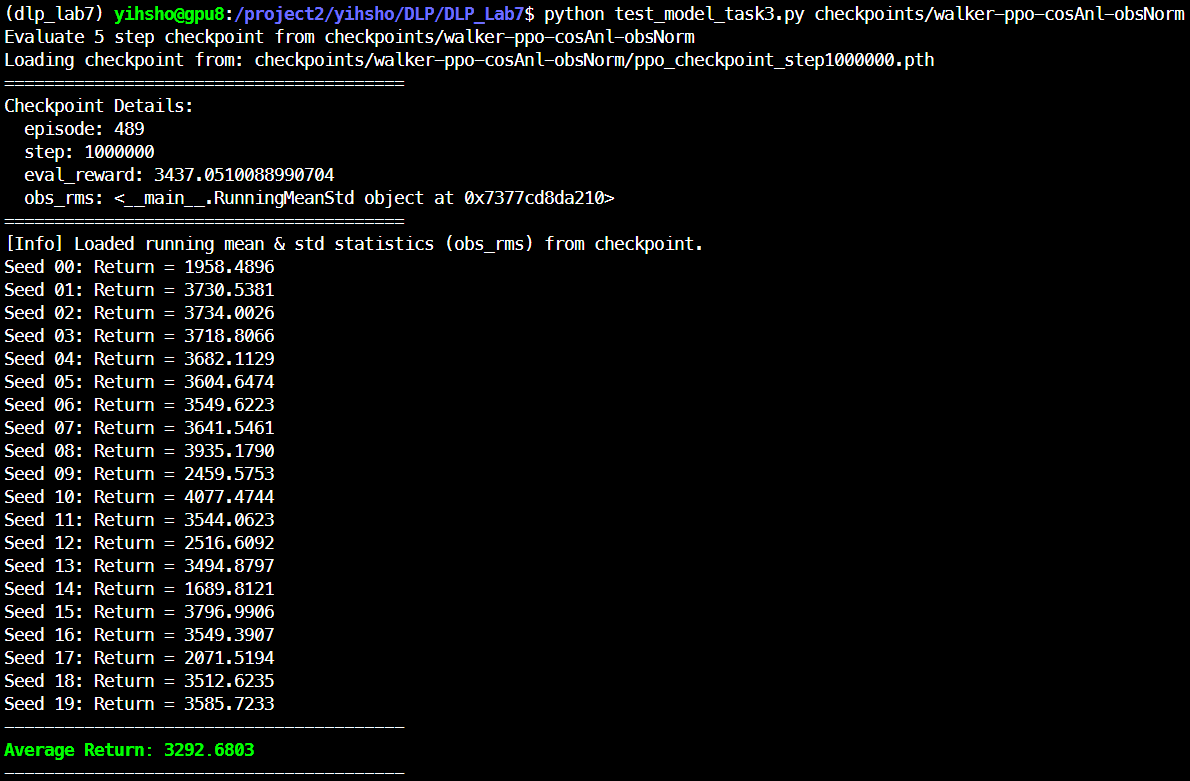
\includegraphics[width=0.48\linewidth]{assets/task3_eval_1M.png}
  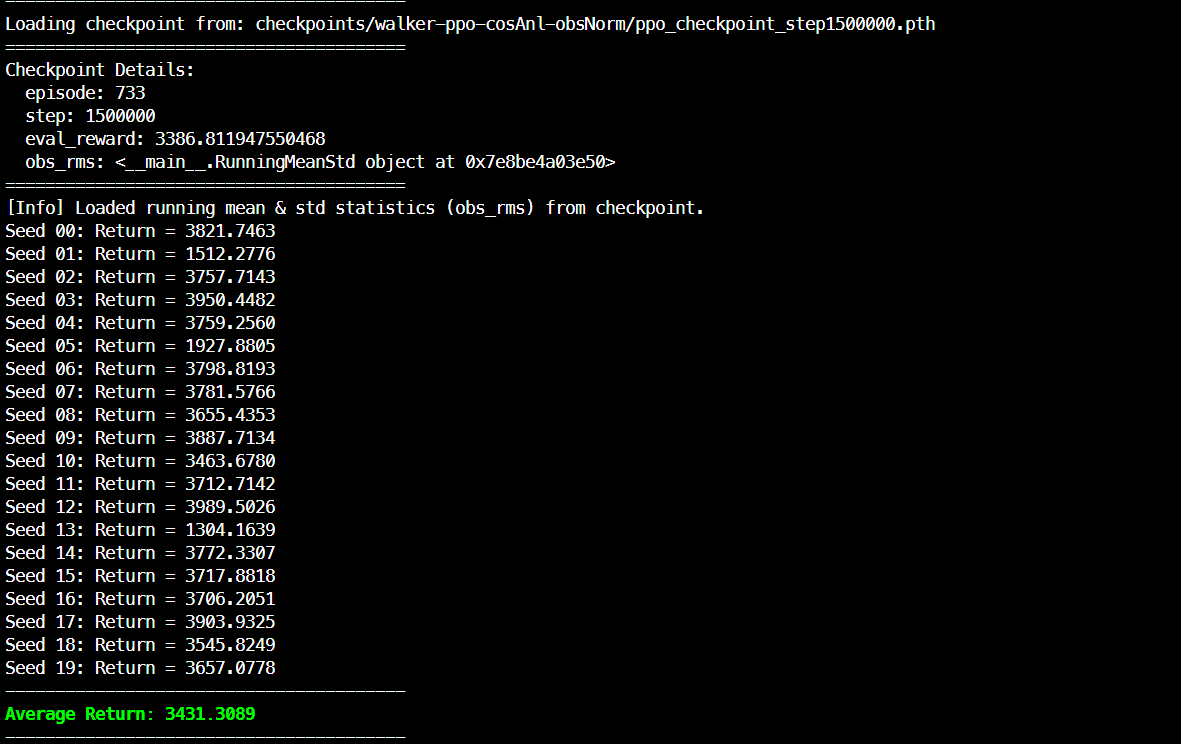
\includegraphics[width=0.48\linewidth]{assets/task3_eval_1.5M.png}
  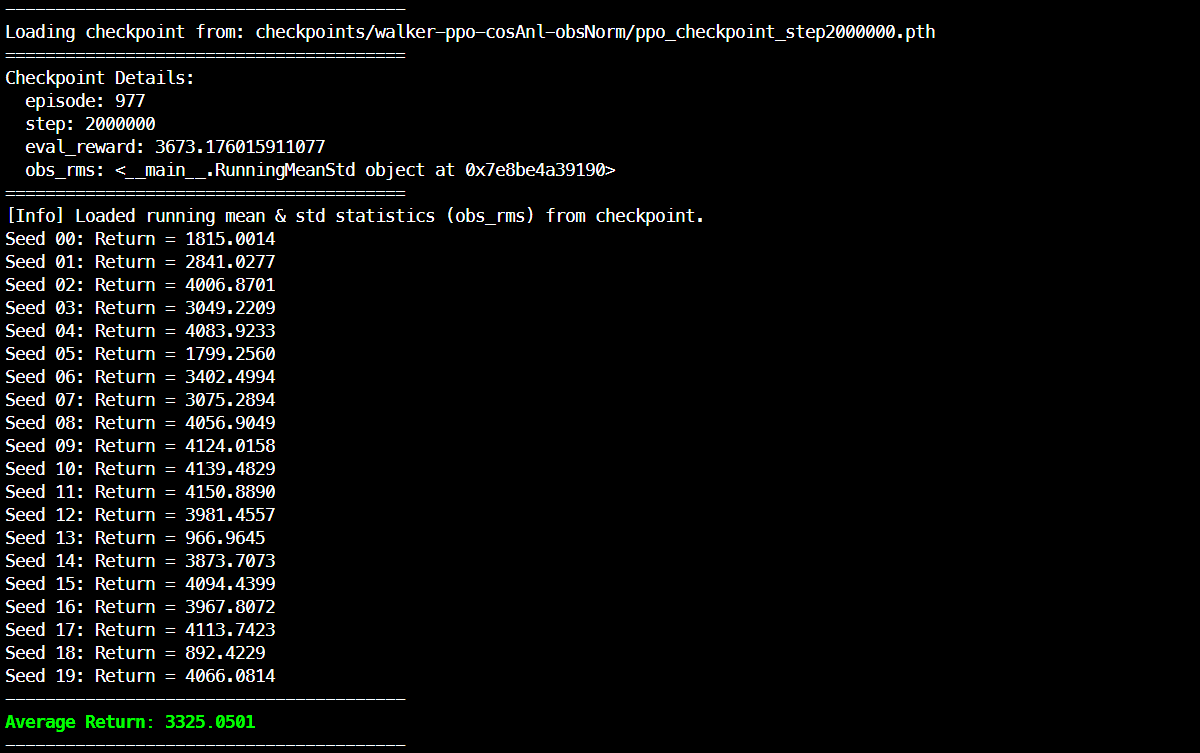
\includegraphics[width=0.48\linewidth]{assets/task3_eval_2M.png}
  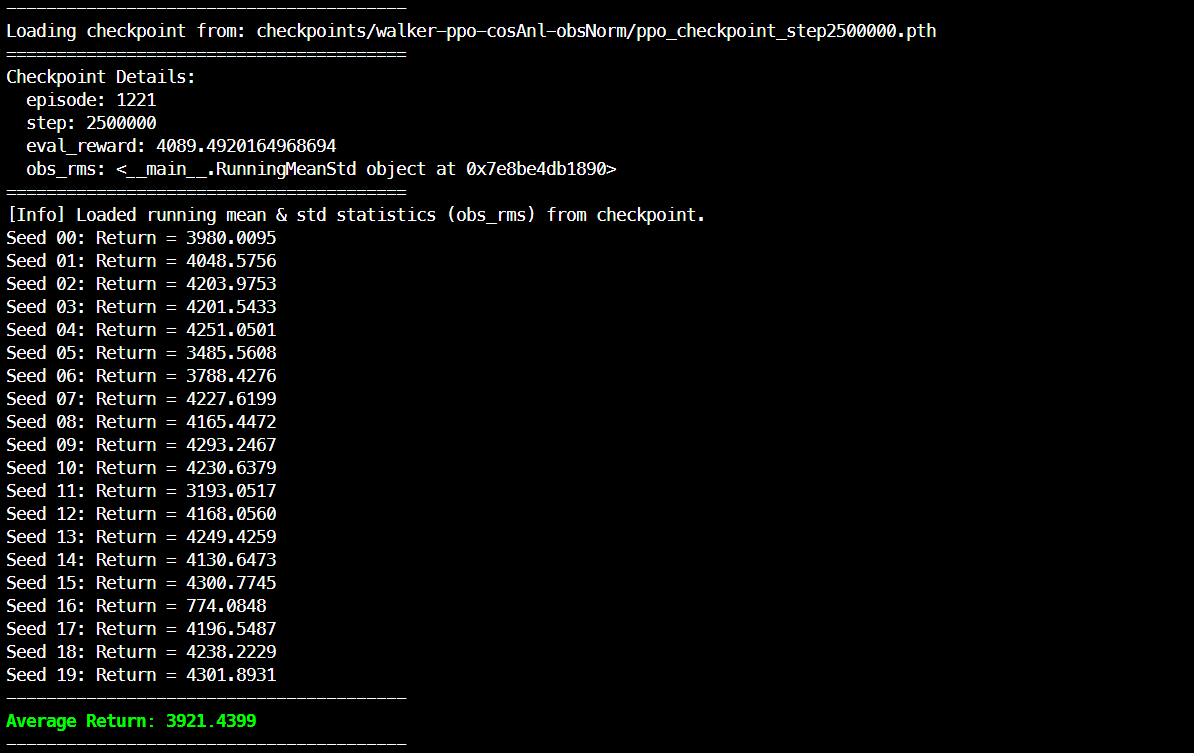
\includegraphics[width=0.48\linewidth]{assets/task3_eval_2.5M.png}
  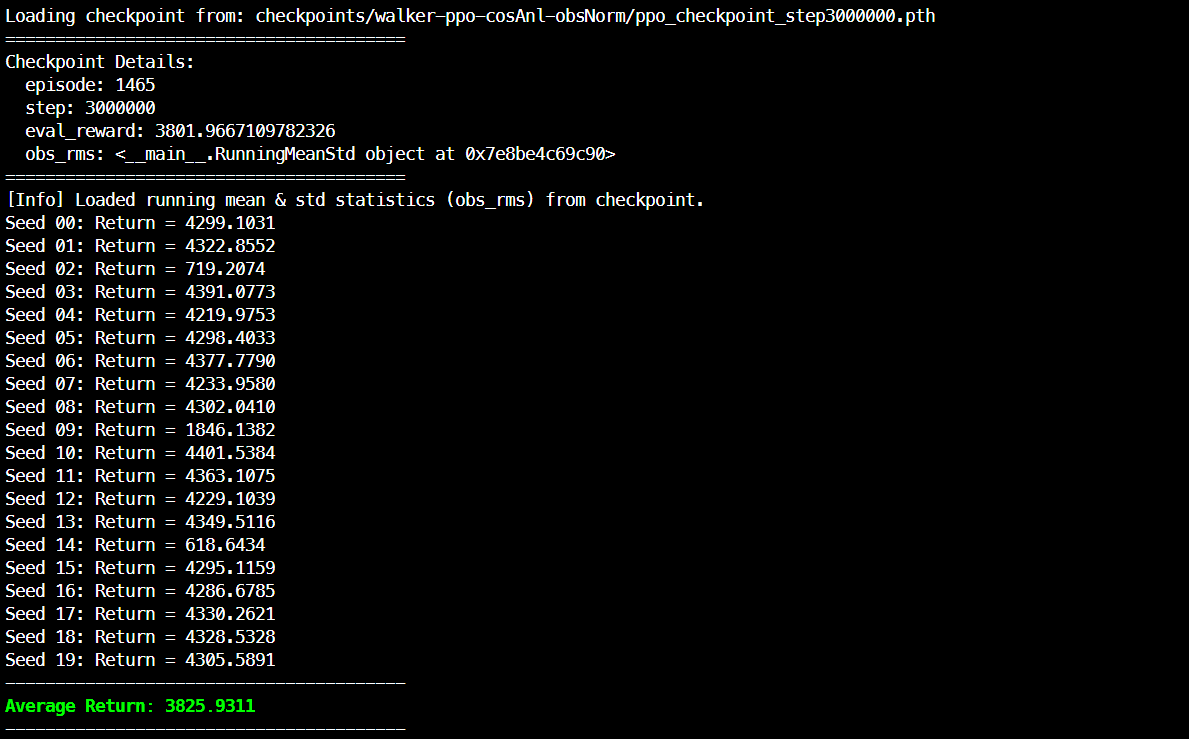
\includegraphics[width=0.48\linewidth]{assets/task3_eval_3M.png}
  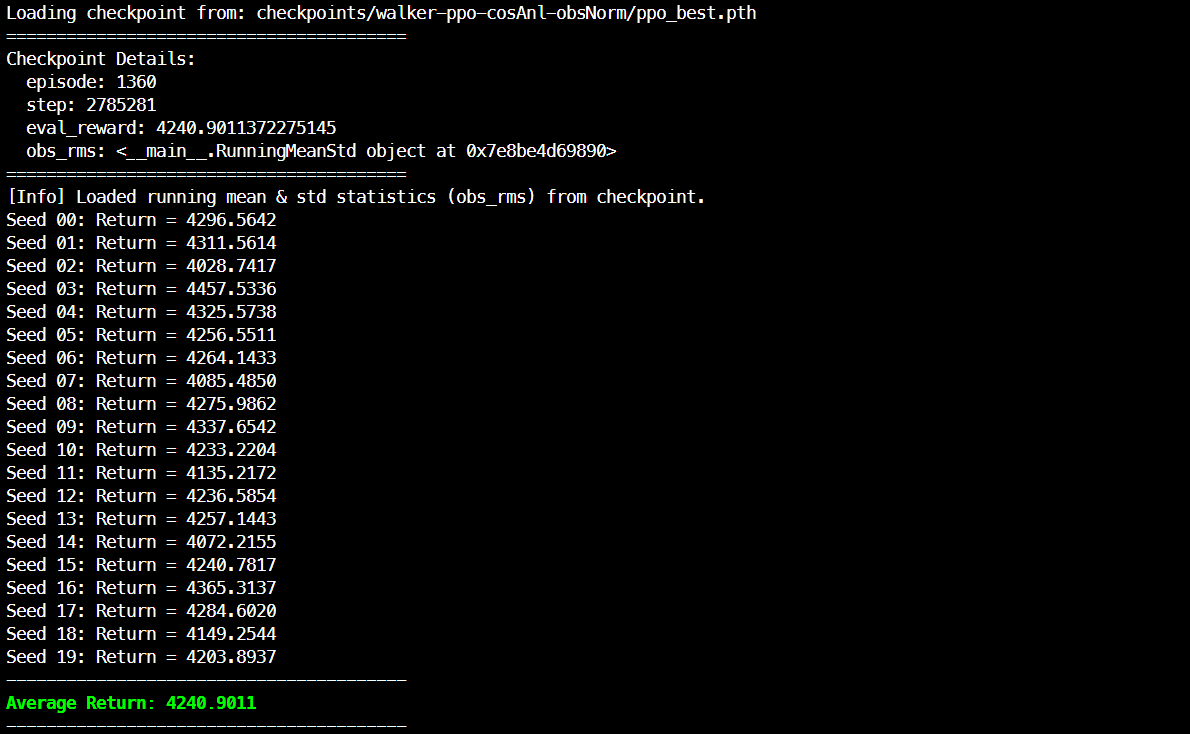
\includegraphics[width=0.48\linewidth]{assets/task3_eval_best.png}
  \caption{\textbf{PPO Walker2d-v5} evaluation terminal output. The
    checkpoints are stored at step 1M, 1.5M, 2M, 2.5M, 3M, and best.}
  \label{fig:task3_eval}
\end{figure}

\begin{table}[H]
  \centering
  \setlength{\tabcolsep}{5pt}
  \begin{tabular}{@{}lcccccc@{}}
    \toprule
    \textbf{Method} & \textbf{1M} & \textbf{1.5M} & \textbf{2M} & \textbf{2.5M} & \textbf{3M} & \textbf{best} \\
    \midrule
    PPO             & 3292        & 3431          & 3325        & 3921          & 3825        & 4240          \\
    \bottomrule
  \end{tabular}
  \caption{\textbf{PPO Walker2d-v5} average return in different
    training steps. It is tested with 20 random seed for each step.}
  \label{tab:task3_eval}
\end{table}


\subsection{Comparison of Sample Efficiency and Training Stability}
\label{subsec:comparison}

\begin{figure}[H]
  \centering
  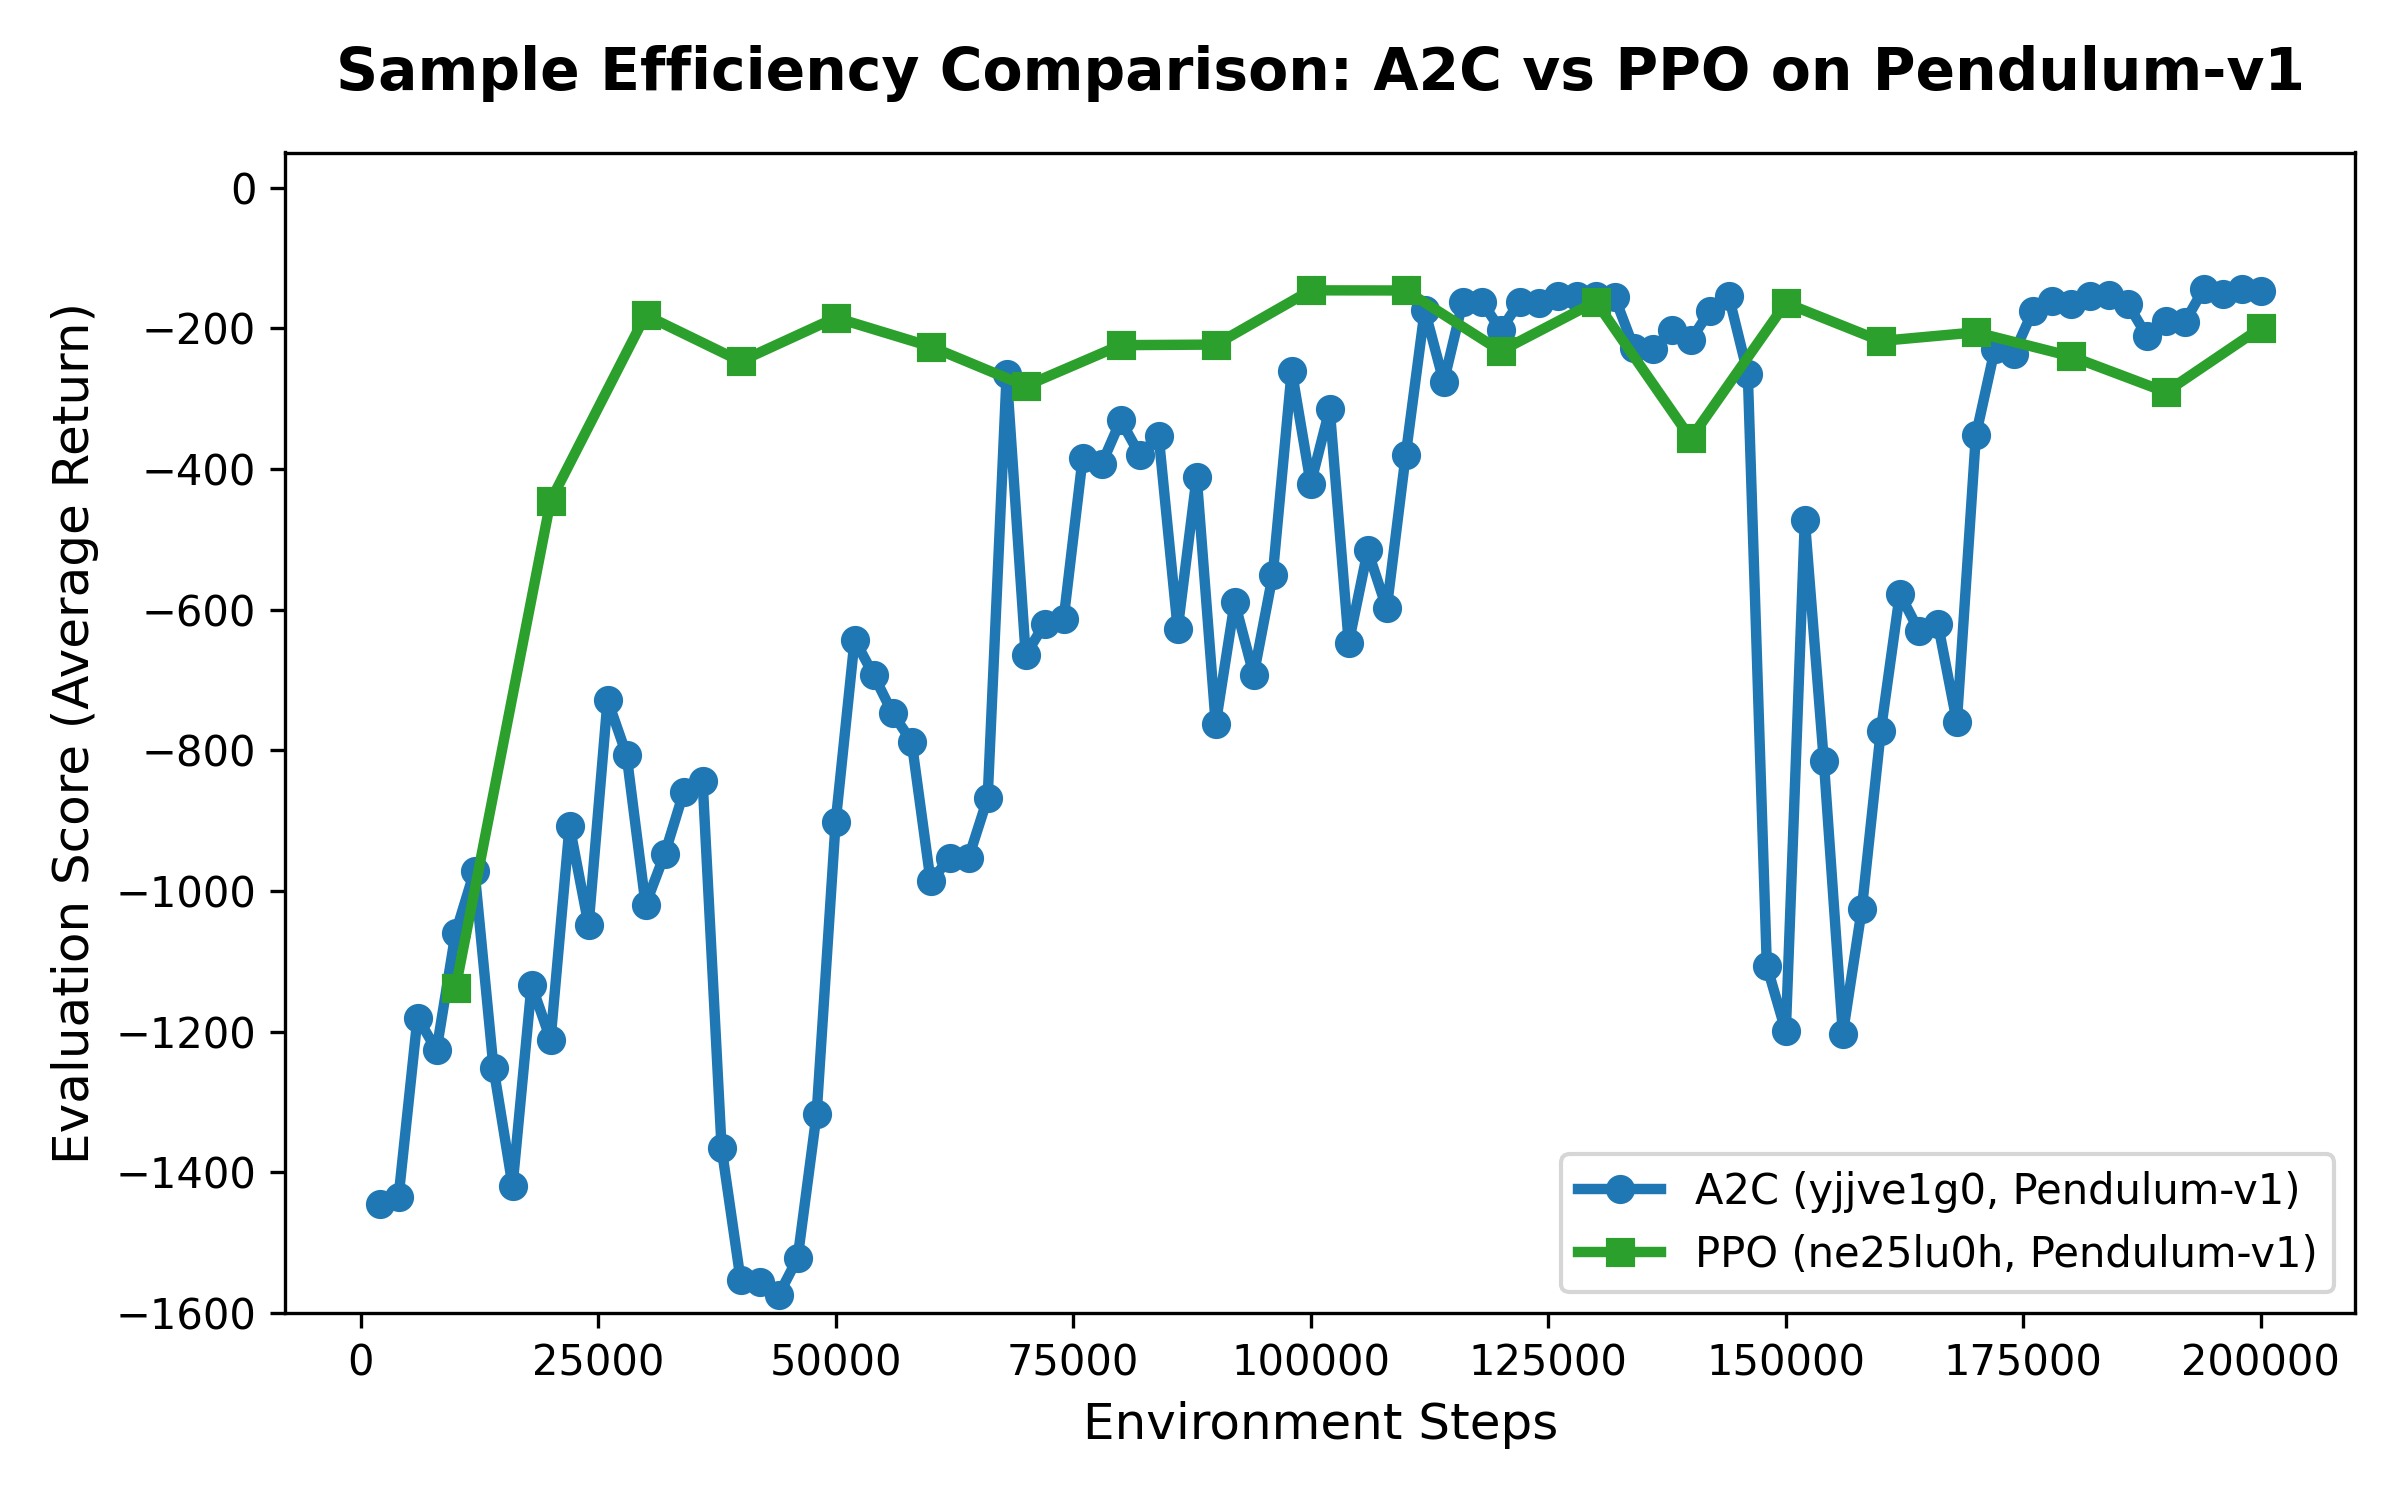
\includegraphics[width=0.95\linewidth]{assets/sample_efficiency.png}
  \caption{\textbf{Sample Efficiency Comparison} of A2C vs. PPO.}
  \label{fig:sample_eff}
\end{figure}

\textbf{Sample Efficiency}: PPO is immensely more sample-efficient than A2C.
A2C is a purely single-step method (TD(0)) that computes gradient updates and
immediately discards transition samples. PPO, however, utilizes a rollout buffer
that stores transitions. It then performs multiple epochs (\verb|update_epoch = 10|)
of optimization on these stored transitions using mini-batch gradient descent.
Furthermore, PPO's GAE advantage estimator ($\tau=0.95$) provides a much
lower-variance target compared to A2C's high-variance single-step TD error,
allowing the policy to learn much faster per environment sample.
As illustrated in \cref{fig:sample_eff}, both agents achieve stable convergence
within 200k steps, with PPO showing faster initial policy optimization but A2C
ultimately reaching a competitive evaluation return under robust exploration.

\textbf{Training Stability}: A2C suffers from high training instability and is
highly susceptible to policy collapse. Because A2C's updates do not restrict the
policy update size, a single outlier gradient step can severely distort the
policy, causing it to become highly deterministic in a suboptimal state. This is
reflected in A2C's highly volatile training curves with frequent performance
drops in \cref{fig:sample_eff}. Conversely, PPO-Clip guarantees stable, monotonic
policy improvements because its clipped surrogate objective bounds the ratio
$r_t(\theta)$ within $[1-\epsilon, 1+\epsilon]$. This prevents catastrophic policy
changes, maintaining a smooth and stable training trajectory.


\subsection{Empirical Parameter Study}
\label{subsec:param_study}

I conducted ablation studies on PPO's clipping parameter $\epsilon$ and the policy
entropy coefficient $c_e$ on the high-dimensional Walker2d-v5 environment
over 3 million environment steps. For all runs, the all continuous control tricks
(observation normalization, advantage normalization, and cosine learning rate
scheduling) were enabled to isolate the impact of the policy optimization
boundaries and exploration weights.

\paragraph{Clipping Parameter ($\epsilon$):}
The clipping parameter $\epsilon$ dictates the boundary of policy updates. I evaluated $\epsilon \in \{0.05, 0.20, 0.50, 1.00\}$, with the evaluation results summarized in \cref{tab:param_study_clip}. Bounding updates too tightly ($\epsilon = 0.05$) ensures high stability but slows down early-stage learning, although it ultimately converges to a highly competitive score. The optimal setting ($\epsilon = 0.20$) balances stability and convergence speed, yielding the fastest learning progress. Relaxing the constraint further ($\epsilon = 0.50$ and $1.00$) severely degrades performance, leading to high training instability, early policy collapse, and significantly lower returns.

\begin{table}[H]
  \centering
  \setlength{\tabcolsep}{4.5pt}
  \begin{tabular}{@{}lccccccc@{}}
    \toprule
    \textbf{Clipping ($\epsilon$)} & \textbf{1M}   & \textbf{1.5M} & \textbf{2M}   & \textbf{2.5M} & \textbf{3M}   & \textbf{best} \\
    \midrule
    0.05                           & 910           & 1739          & \textbf{3545} & \textbf{4107} & \textbf{4143} & 4313 \\
    0.20                           & \textbf{2924} & \textbf{2979} & 2791          & 3978          & 3901          & \textbf{4367} \\
    0.50                           & 1754          & 2171          & 2451          & 3099          & 3274          & 3414          \\
    1.00                           & 293           & 540           & 627           & 2451          & 2033          & 2472          \\
    \bottomrule
  \end{tabular}
  \caption{\textbf{Clipping parameter ablation} average evaluation return at
    different training steps on Walker2d-v5. The best result in each time steps
    is marked inn bold.}
  \label{tab:param_study_clip}
\end{table}

\begin{figure}[H]
  \centering
  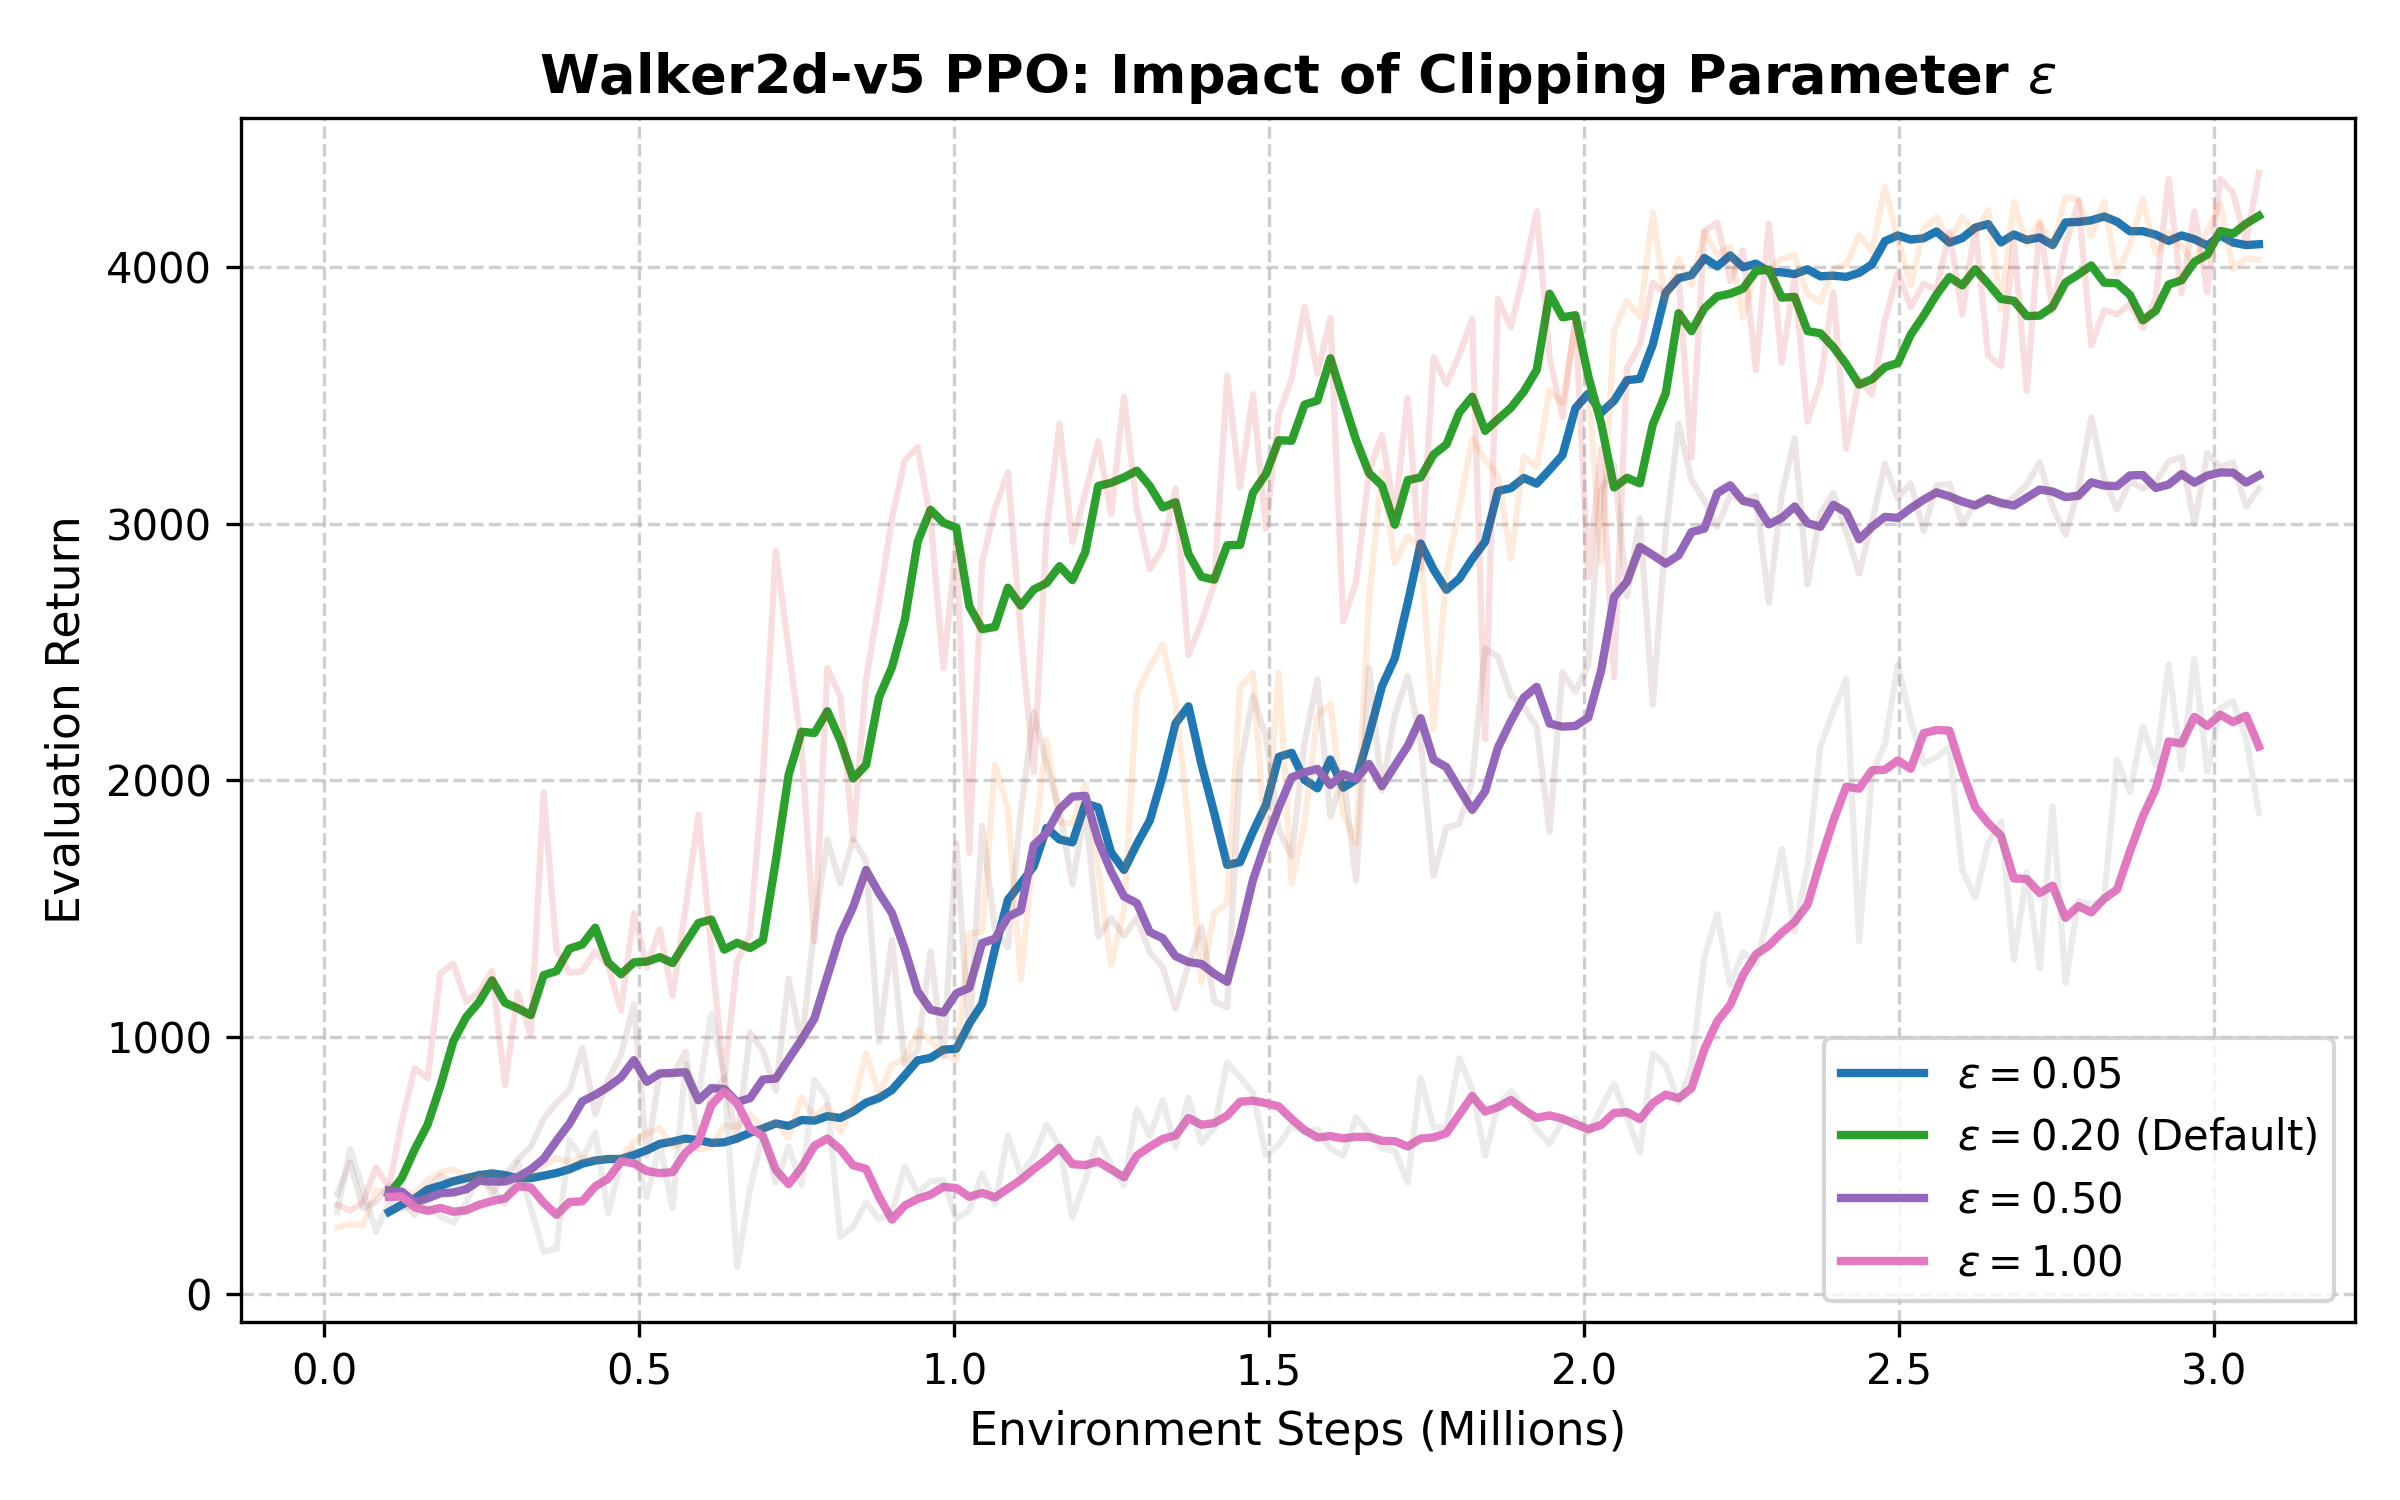
\includegraphics[width=0.95\linewidth]{assets/param_study_clip.png}
  \caption{\textbf{Clipping parameter ablation}. Solid curves represent
    the smoothed evaluation returns using a simple moving average with
    a window size of 5, while the raw unsmoothed curves are plotted faintly
    in the background. Bounding updates too tightly ($\epsilon = 0.05$)
    limits initial learning progress, while excessively loose boundaries
    ($\epsilon = 1.00$) lead to highly suboptimal behaviors.}
  \label{fig:param_study_clip}
\end{figure}

\paragraph{Entropy Coefficient ($c_e$):}
The entropy coefficient $c_e$ regulates the exploration-exploitation trade-off. I evaluated $c_e \in \{0.00, 0.001, 0.01, 0.10\}$, with the performance metrics documented in \cref{tab:param_study_entropy}. Without sufficient entropy regularization ($c_e = 0.00$ and $0.001$), the policy quickly collapses to a near-deterministic state and gets trapped in suboptimal gaits. While the moderate value ($c_e = 0.01$) enables smooth gait learning, the high entropy coefficient ($c_e = 0.10$) delivers the absolute best performance. This demonstrates that high-dimensional locomotion environments benefit significantly from persistent exploration pressure to discover highly efficient walking gaits.

\begin{table}[H]
  \centering
  \setlength{\tabcolsep}{4.5pt}
  \begin{tabular}{@{}lccccccc@{}}
    \toprule
    \textbf{Entropy ($c_e$)} & \textbf{1M}   & \textbf{1.5M} & \textbf{2M}   & \textbf{2.5M} & \textbf{3M}   & \textbf{best} \\
    \midrule
    0.00                     & 2676          & 2678          & 3203          & 4025          & 3752          & 4151          \\
    0.001                    & 1896          & 2214          & 2640          & 3346          & 3758          & 3956          \\
    0.01                     & 2924          & 2979          & 2791          & 3978          & 3901          & 4367          \\
    0.10                     & \textbf{4136} & \textbf{4385} & \textbf{4924} & \textbf{5490} & \textbf{5345} & \textbf{5693} \\
    \bottomrule
  \end{tabular}
  \caption{\textbf{Entropy coefficient ablation} average evaluation return at
    different training steps on Walker2d-v5. The best result in each time steps
    is marked in bold.}
  \label{tab:param_study_entropy}
\end{table}

\begin{figure}[H]
  \centering
  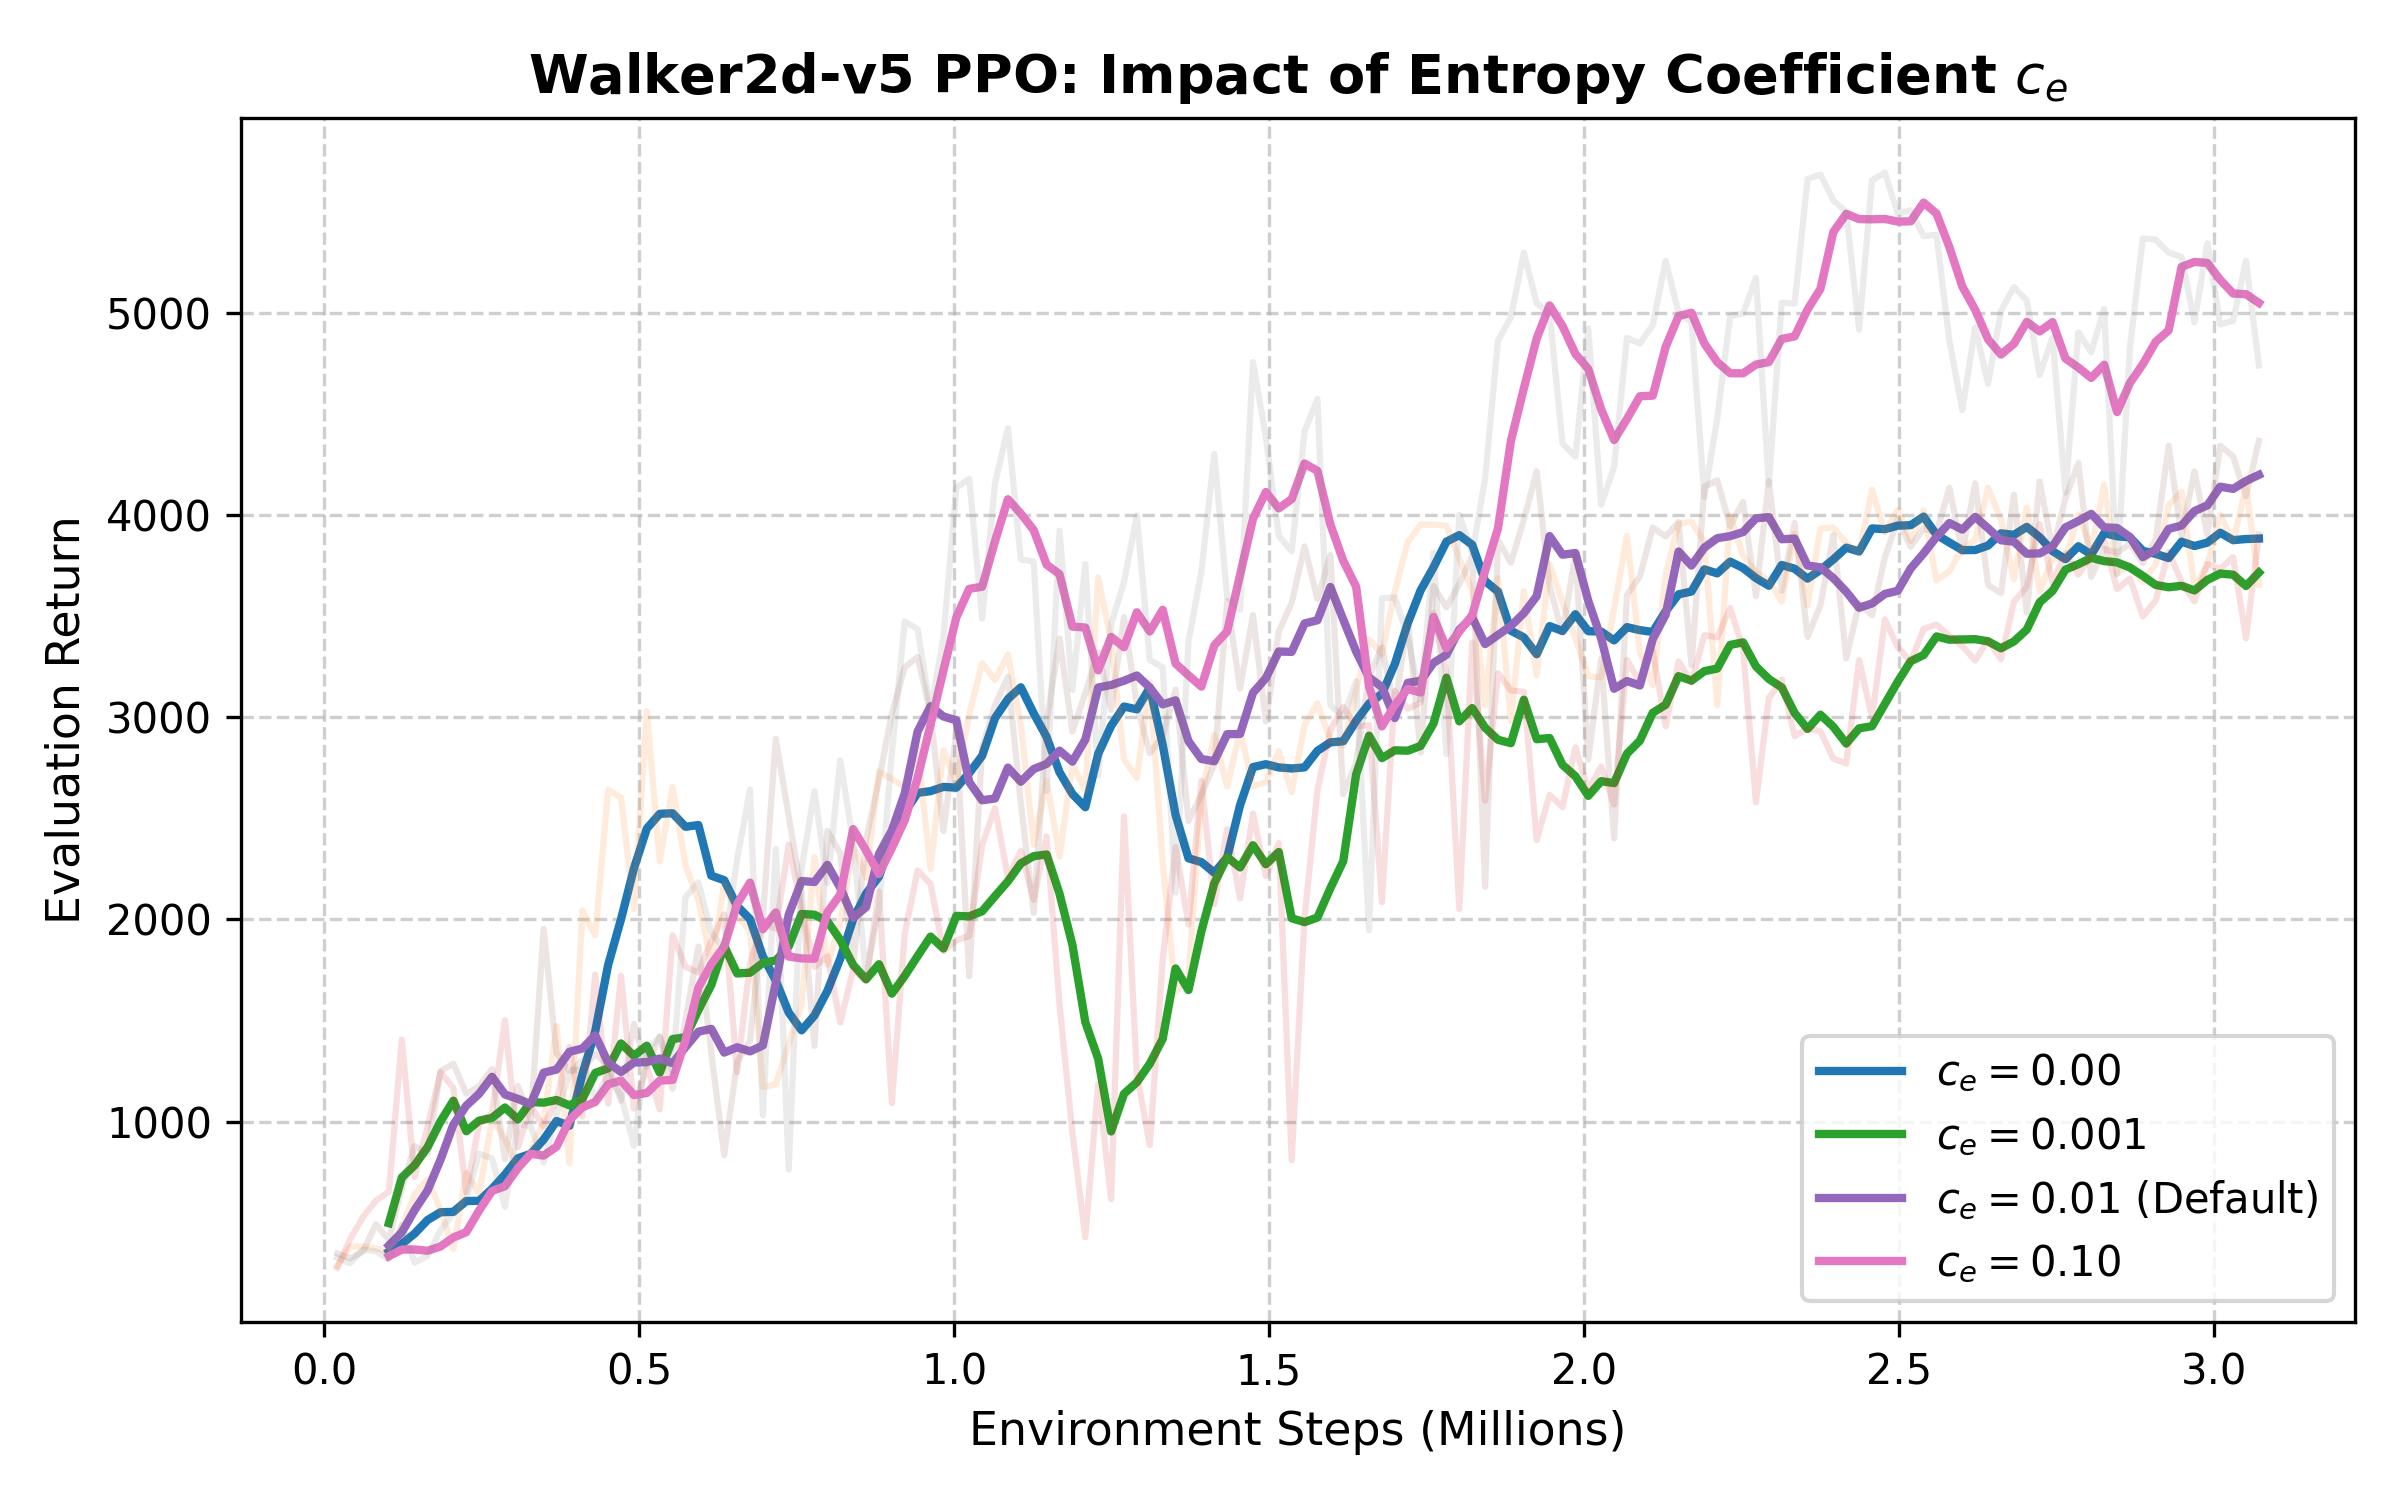
\includegraphics[width=0.95\linewidth]{assets/param_study_entropy.png}
  \caption{\textbf{Entropy coefficient ablation}. Solid curves represent
    the smoothed evaluation returns using a simple moving average with
    a window size of 5, while raw curves are plotted faintly
    in the background. A higher entropy weight ($c_e = 0.10$) promotes
    robust exploration, yielding a substantial performance boost in the
    complex Walker2d locomotion task, whereas too little entropy leads to
    premature convergence in local optima.}
  \label{fig:param_study_entropy}
\end{figure}

\section{Additional Analysis: Ablation Study on Continuous Control Optimizations}
\label{sec:analysis_bonus}

To analyze the impact of individual continuous control optimization strategies,
I conducted comprehensive ablation experiments on the Walker2d-v5 environment.
The first study (\cref{fig:task3_ablation_add}) investigates the effect of adding
each trick individually to Vanilla PPO, while the second study
(\cref{fig:task3_ablation_sub}) examines the performance degradation when
individual tricks are subtracted from the full configuration.

\begin{figure}[H]
  \centering
  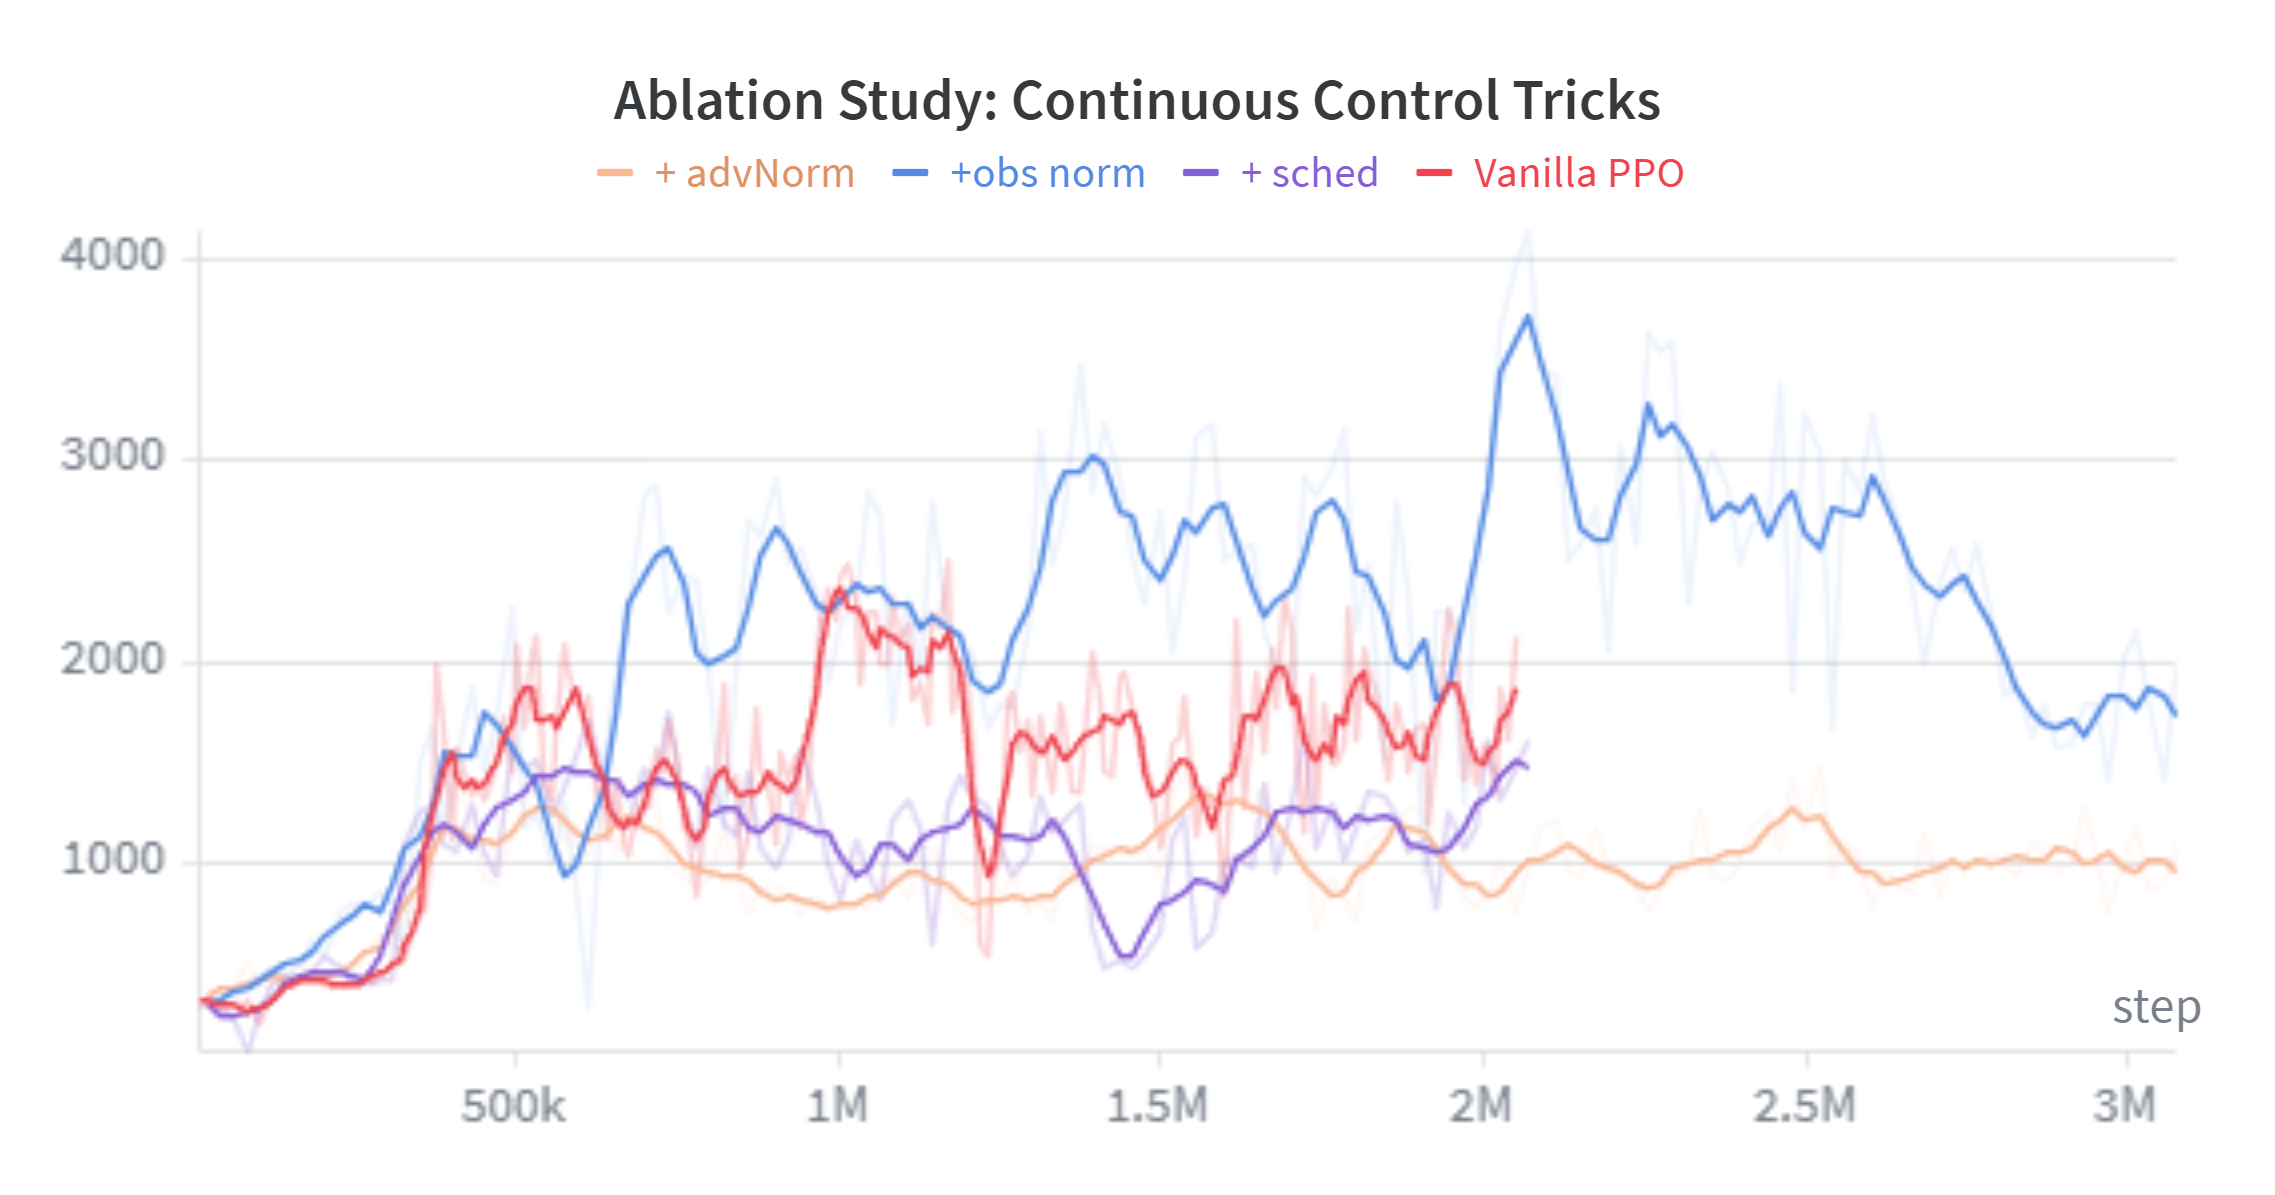
\includegraphics[width=1\linewidth]{assets/abla_bonus_add.png}
  \caption{\textbf{Adding individual continuous control tricks to Vanilla PPO}.}
  \label{fig:task3_ablation_add}
\end{figure}

The ``Adding'' study (\cref{fig:task3_ablation_add}) reveals that
Observation Normalization (\verb|+obs norm|) is the single most critical
individual factor for successful policy optimization. Adding only observation
normalization enables PPO to achieve a rapid, substantial performance surge,
peaking near a return of $3700$ around 2.1M steps. This is because standardizing
the high-dimensional Walker2d observations to zero-mean and unit variance
prevents gradient saturation in early layers. In contrast, adding only learning
rate scheduling (\verb|+sched|) or only advantage normalization (\verb|+advNorm|)
in isolation fails to overcome the state-scaling bottleneck, resulting in worse
performance than vanilla PPO. However, the solitary \verb|+obs norm| run also
highlights its limitations: without learning rate annealing or mini-batch
stabilization, the policy suffers from late-stage training instability, 
and decays back to approximately $1800$ by 3M steps.

\begin{figure}[H]
  \centering
  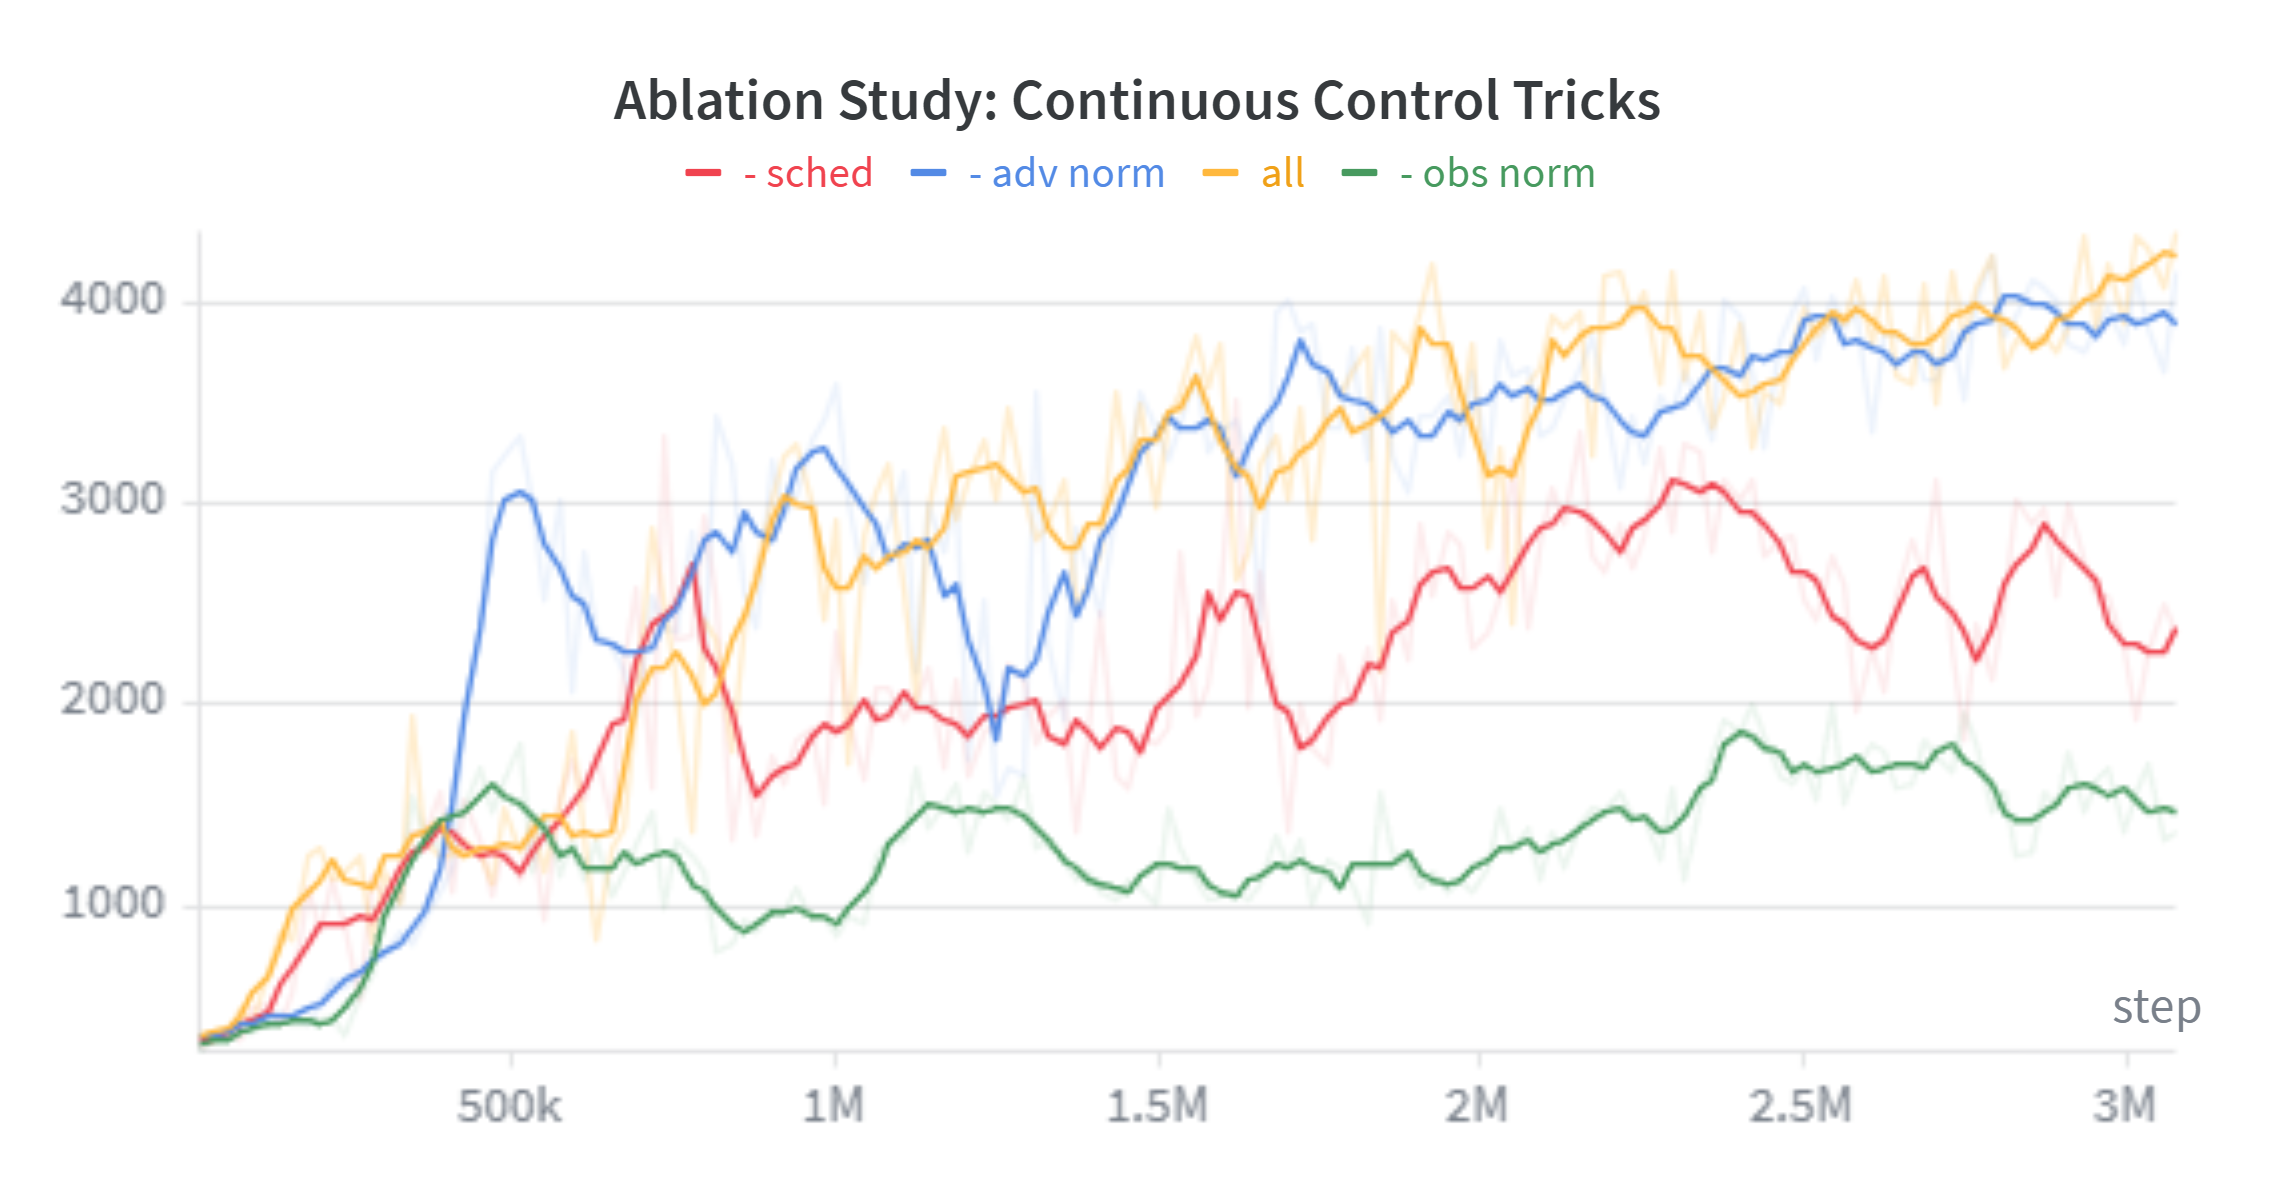
\includegraphics[width=1\linewidth]{assets/abla_bonus_sub.png}
  \caption{\textbf{Subtracting individual continuous control tricks from the
    full configuration}.}
  \label{fig:task3_ablation_sub}
\end{figure}

The ``Subtracting'' study (\cref{fig:task3_ablation_sub}) confirms the
synergistic necessity of all three optimizations. The full configuration
(\verb|all|), combining all three tricks, achieves the highest return
with highly stable, monotonic growth. In contrast, removing observation
normalization (\verb|-obs norm|) causes a catastrophic drop, pinning
performance below $1800$ and demonstrating its role as the absolute
cornerstone. Removing the learning rate scheduler (\verb|-sched|) allows efficient
early learning but results in a mid-stage peak near $3100$ followed by a
steady decay to $2400$, illustrating the necessity of learning rate annealing
to prevent late-stage policy degradation. Lastly, while removing advantage
normalization (\verb|-adv norm|) yields rapid early acceleration (reaching
$3000$ at 500k steps) and a competitive final return of $3900$, it exhibits
larger training variance and slightly lower asymptotic performance, highlighting
its vital role in mini-batch stabilization.

\section{Conclusion}
\label{sec:conclusion}

In this lab, I successfully implemented and analyzed policy-based reinforcement
learning using A2C and PPO. The experimental evaluations on Pendulum-v1
highlight that PPO-Clip offers significantly higher sample efficiency and
exceptional training stability compared to A2C, which is highly prone to gradient
volatility and suboptimal policy convergence. Furthermore, scaling PPO to the
high-dimensional Walker2d-v5 environment demonstrates that observation
normalization, advantage normalization, and cosine learning rate scheduling are
indispensable continuous control strategies. This lab successfully highlights the
importance of matching robust loss formulation with proper state conditioning
and stabilization tricks to achieve state-of-the-art continuous control
performance.

\end{document}